\documentclass[10pt,xcolor=dvipsnames]{beamer}\usepackage[]{graphicx}\usepackage[]{color}
%% maxwidth is the original width if it is less than linewidth
%% otherwise use linewidth (to make sure the graphics do not exceed the margin)
\makeatletter
\def\maxwidth{ %
  \ifdim\Gin@nat@width>\linewidth
    \linewidth
  \else
    \Gin@nat@width
  \fi
}
\makeatother

\definecolor{fgcolor}{rgb}{0.345, 0.345, 0.345}
\newcommand{\hlnum}[1]{\textcolor[rgb]{0.686,0.059,0.569}{#1}}%
\newcommand{\hlstr}[1]{\textcolor[rgb]{0.192,0.494,0.8}{#1}}%
\newcommand{\hlcom}[1]{\textcolor[rgb]{0.678,0.584,0.686}{\textit{#1}}}%
\newcommand{\hlopt}[1]{\textcolor[rgb]{0,0,0}{#1}}%
\newcommand{\hlstd}[1]{\textcolor[rgb]{0.345,0.345,0.345}{#1}}%
\newcommand{\hlkwa}[1]{\textcolor[rgb]{0.161,0.373,0.58}{\textbf{#1}}}%
\newcommand{\hlkwb}[1]{\textcolor[rgb]{0.69,0.353,0.396}{#1}}%
\newcommand{\hlkwc}[1]{\textcolor[rgb]{0.333,0.667,0.333}{#1}}%
\newcommand{\hlkwd}[1]{\textcolor[rgb]{0.737,0.353,0.396}{\textbf{#1}}}%
\let\hlipl\hlkwb

\usepackage{framed}
\makeatletter
\newenvironment{kframe}{%
 \def\at@end@of@kframe{}%
 \ifinner\ifhmode%
  \def\at@end@of@kframe{\end{minipage}}%
  \begin{minipage}{\columnwidth}%
 \fi\fi%
 \def\FrameCommand##1{\hskip\@totalleftmargin \hskip-\fboxsep
 \colorbox{shadecolor}{##1}\hskip-\fboxsep
     % There is no \\@totalrightmargin, so:
     \hskip-\linewidth \hskip-\@totalleftmargin \hskip\columnwidth}%
 \MakeFramed {\advance\hsize-\width
   \@totalleftmargin\z@ \linewidth\hsize
   \@setminipage}}%
 {\par\unskip\endMakeFramed%
 \at@end@of@kframe}
\makeatother

\definecolor{shadecolor}{rgb}{.97, .97, .97}
\definecolor{messagecolor}{rgb}{0, 0, 0}
\definecolor{warningcolor}{rgb}{1, 0, 1}
\definecolor{errorcolor}{rgb}{1, 0, 0}
\newenvironment{knitrout}{}{} % an empty environment to be redefined in TeX

\usepackage{alltt}
\setbeamertemplate{navigation symbols}{}



\usepackage{color}
\usepackage{CREAL_slides}
\usepackage[latin1]{inputenc} 
\usepackage{calc} 
\usepackage[loadonly]{enumitem}
\usepackage{float}
\usepackage[position=top,singlelinecheck=off]{subfig}

\DeclareMathOperator{\argmax}{arg\,max} 







\title[Omic data analysis]{Multi-omic data analysis}
\author[Juan R Gonzalez]{Juan R Gonzalez}
\institute[CREAL]{BRGE - Bioinformatics Research Group in Epidemiology \\
		  Barcelona Institute for Global Health (ISGlobal) \\ 
		           {\tt e-mail:juanr.gonzalez@isglobal.org} \\
                  \url{http://www.creal.cat/brge} 
                  }
                 
\date{}
\IfFileExists{upquote.sty}{\usepackage{upquote}}{}
\begin{document}

                            


\frame{\titlepage}

\frame{\tableofcontents}



%%%%%%%%%%%%%%%%%%%%%%%%%%%%%%%%%%%
\section{Introduction}
%%%%%%%%%%%%%%%%%%%%%%%%%%%%%%%%%%%


\begin{frame}\frametitle{Introduction}

\begin{itemize}
\item Undersanding the genetic basis of \textcolor{OliveGreen}{complex traits} is an open question for may researchers
\pause
\item Recent advances in technology has made this problem even more complex by incorporating other pieces
of information such as neuroimaging, daily measurements of enviromental exposures among others
\pause
\item The main challenge is to analyze the vast amount of data that is being generated, particularly how to integrate information from different tables
\end{itemize}
\end{frame}



\begin{frame}\frametitle{Introduction}

\begin{figure}
\begin{center}
 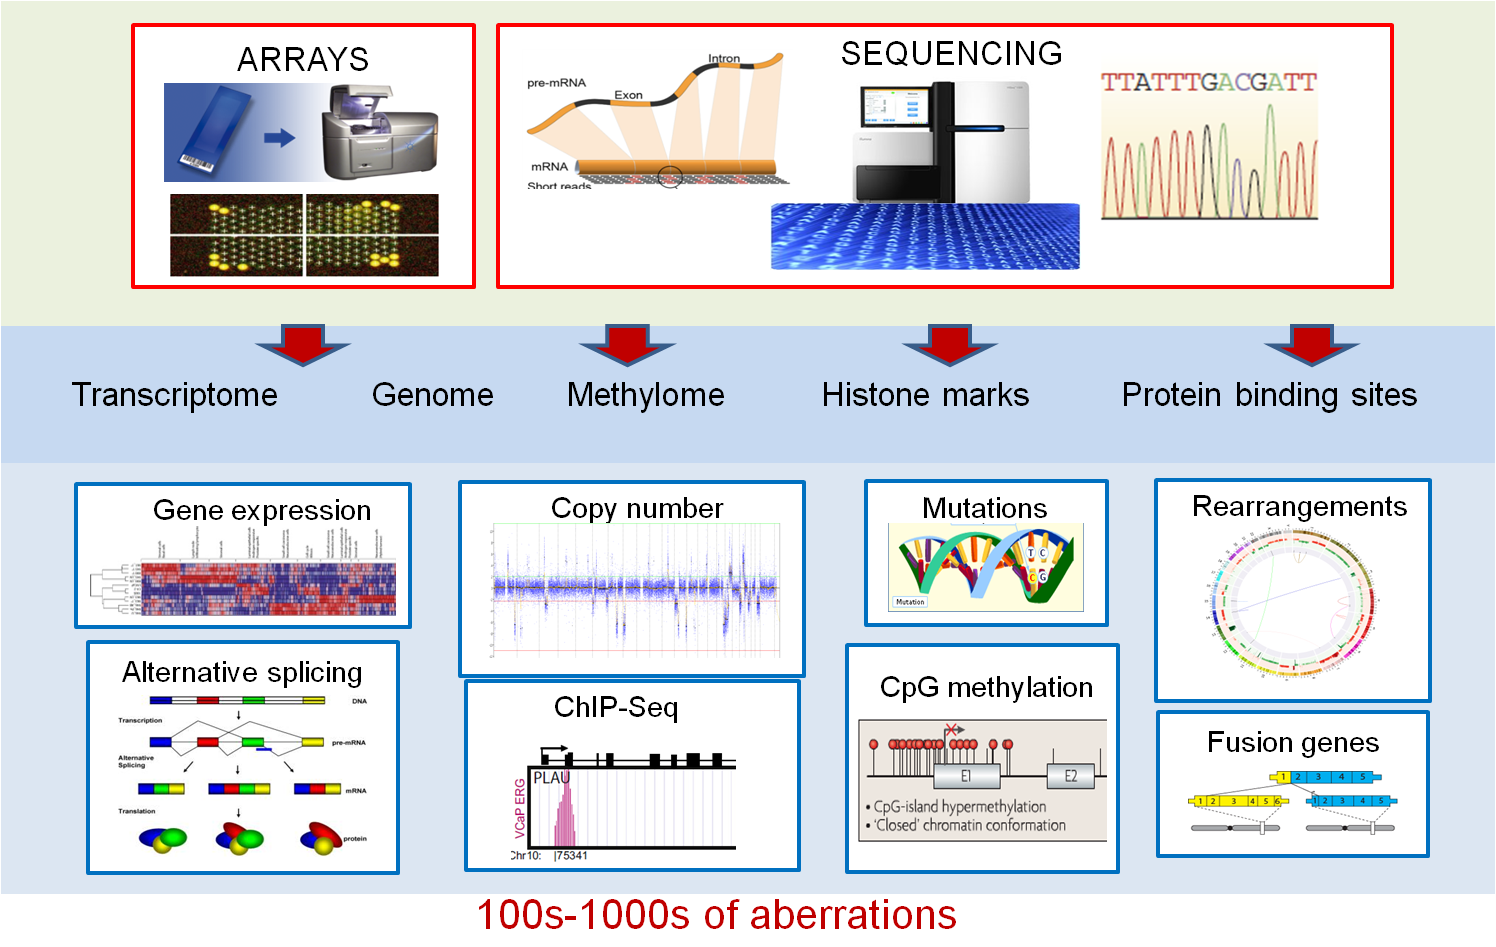
\includegraphics[height=6cm, width=6.5cm]{figures/general_omic_data.png}
\end{center}
\end{figure}

\end{frame}


\begin{frame}\frametitle{Introduction}

\begin{figure}
\begin{center}
 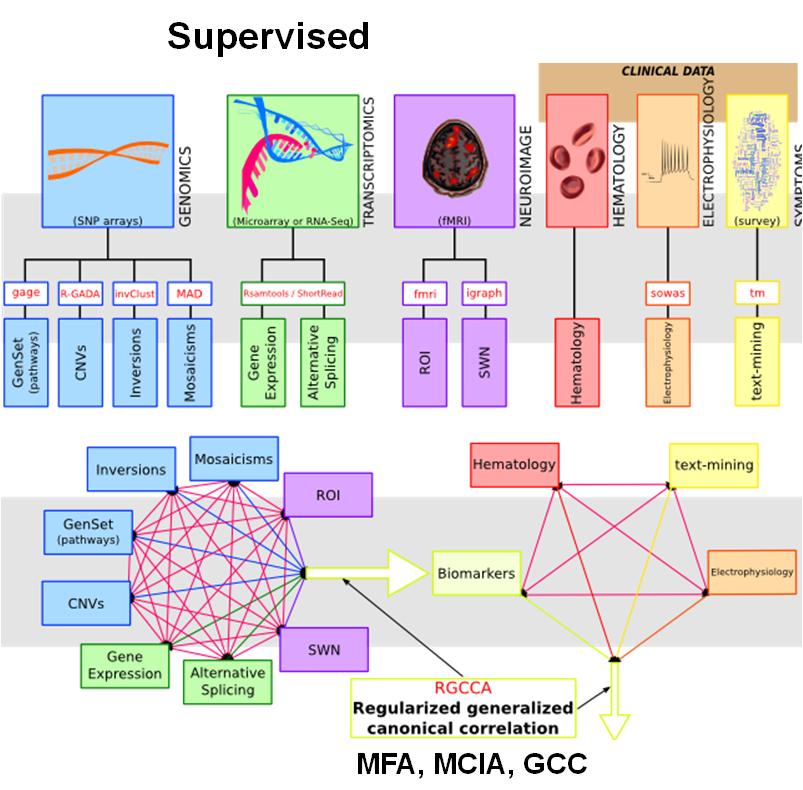
\includegraphics[height=6cm, width=6cm]{figures/supervised_multi_omic.png}
\end{center}
\end{figure}

\end{frame}


%\begin{frame}\frametitle{Introduction}
%\begin{figure}
%\begin{center}
% 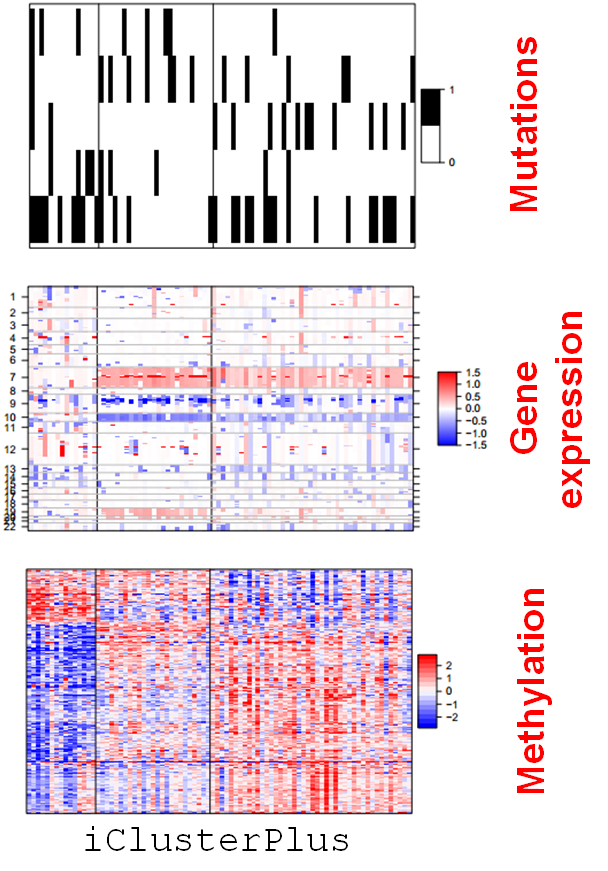
\includegraphics[height=6cm, width=5cm]{figures/non_supervised_multi_omic.png}
%\end{center}
%\end{figure}
%\end{frame}


\begin{frame}\frametitle{Introduction}

\begin{itemize}
\item Data integration (Integrative bioinformatics, integrated 
analysis, crossomics, multi-dataset analysis, data fusion, ...) is being crucial in Bioinformatics/Biology/Epidemiology
\item Data integration may refer to different aspects
  \begin{itemize}
   \item Computational combination of data (sets)
   \item Simultaneous analysis of different variables from different tables, different time points, different tissues, ...
   \item Provide biological insights by using information from existing databases (ENCODE, GTEX, KEGG, ...)
  \end{itemize}
\item Here we mean the process by which different types of omic data are combined as predictor 
variables to allow more thorough and comprehensive modelling of complex traits or phenotypes
\end{itemize}
\end{frame}


\begin{frame}\frametitle{Introduction}

\begin{itemize}
\item \textcolor{OliveGreen}{Multi-staged analysis}: Involves integrating information using a stepwise or hierarchical analysis approach
\item \textcolor{OliveGreen}{Meta-dimensional analysis}: Refers to the concept of integrating multiple different data types to build a multivariate model associated with a given outcome
\end{itemize}
\end{frame}



%%%%%%%%%%%%%%%%%%%%%%%%%%%%%%
\section{Multi-staged analysis}
%%%%%%%%%%%%%%%%%%%%%%%%%%%%%%


\begin{frame}\frametitle{Multi-staged analysis}

\begin{itemize}
\item \textcolor{OliveGreen}{Multi-staged analysis}: Involves integrating information using a stepwise or hierarchical analysis approach
\item \textcolor{Gray}{Meta-dimensional analysis: Refers to the concept of integrating multiple different data types to build a multivariate model associated with a given outcome}
\end{itemize}
\end{frame}


\begin{frame}\frametitle{Multi-staged analysis}
\begin{itemize}
\item \textcolor{OliveGreen}{Genomic variation analysis approaches}: Triangle approach
   \begin{enumerate}
    \item SNPs are associated with the phenotype of interesed and filtered based on p-values
    \item Significant SNPs are tested for association with another level of omic data (i.e eQTLs)
    \item Omic data used in step 2 are then tested for correlation with phenotype of interest
   \end{enumerate}

\pause

\item \textcolor{OliveGreen}{Domain knowledge-guided approaches}: Integration of functional and pathway information
   \begin{enumerate}
    \item Significant results (regions of interest) are annotated in databases such as ENCODE, Roadmap Epigenomic Project, KEGG, ...
    \item We an determine whether those regions are within pathways and/or overlaping with functional units, sucha as transcription factors binding, hyper- or hypo-methylated regions
    \item Overlaping regions are then correlated with the phenotype of interest
    \item The main limitation is that this method is biased by current knowledge
   \end{enumerate}
\end{itemize}
\end{frame}



\begin{frame}\frametitle{Types of multi-staged analyses}

\begin{figure}
  \subfloat[Genomic variation analysis]{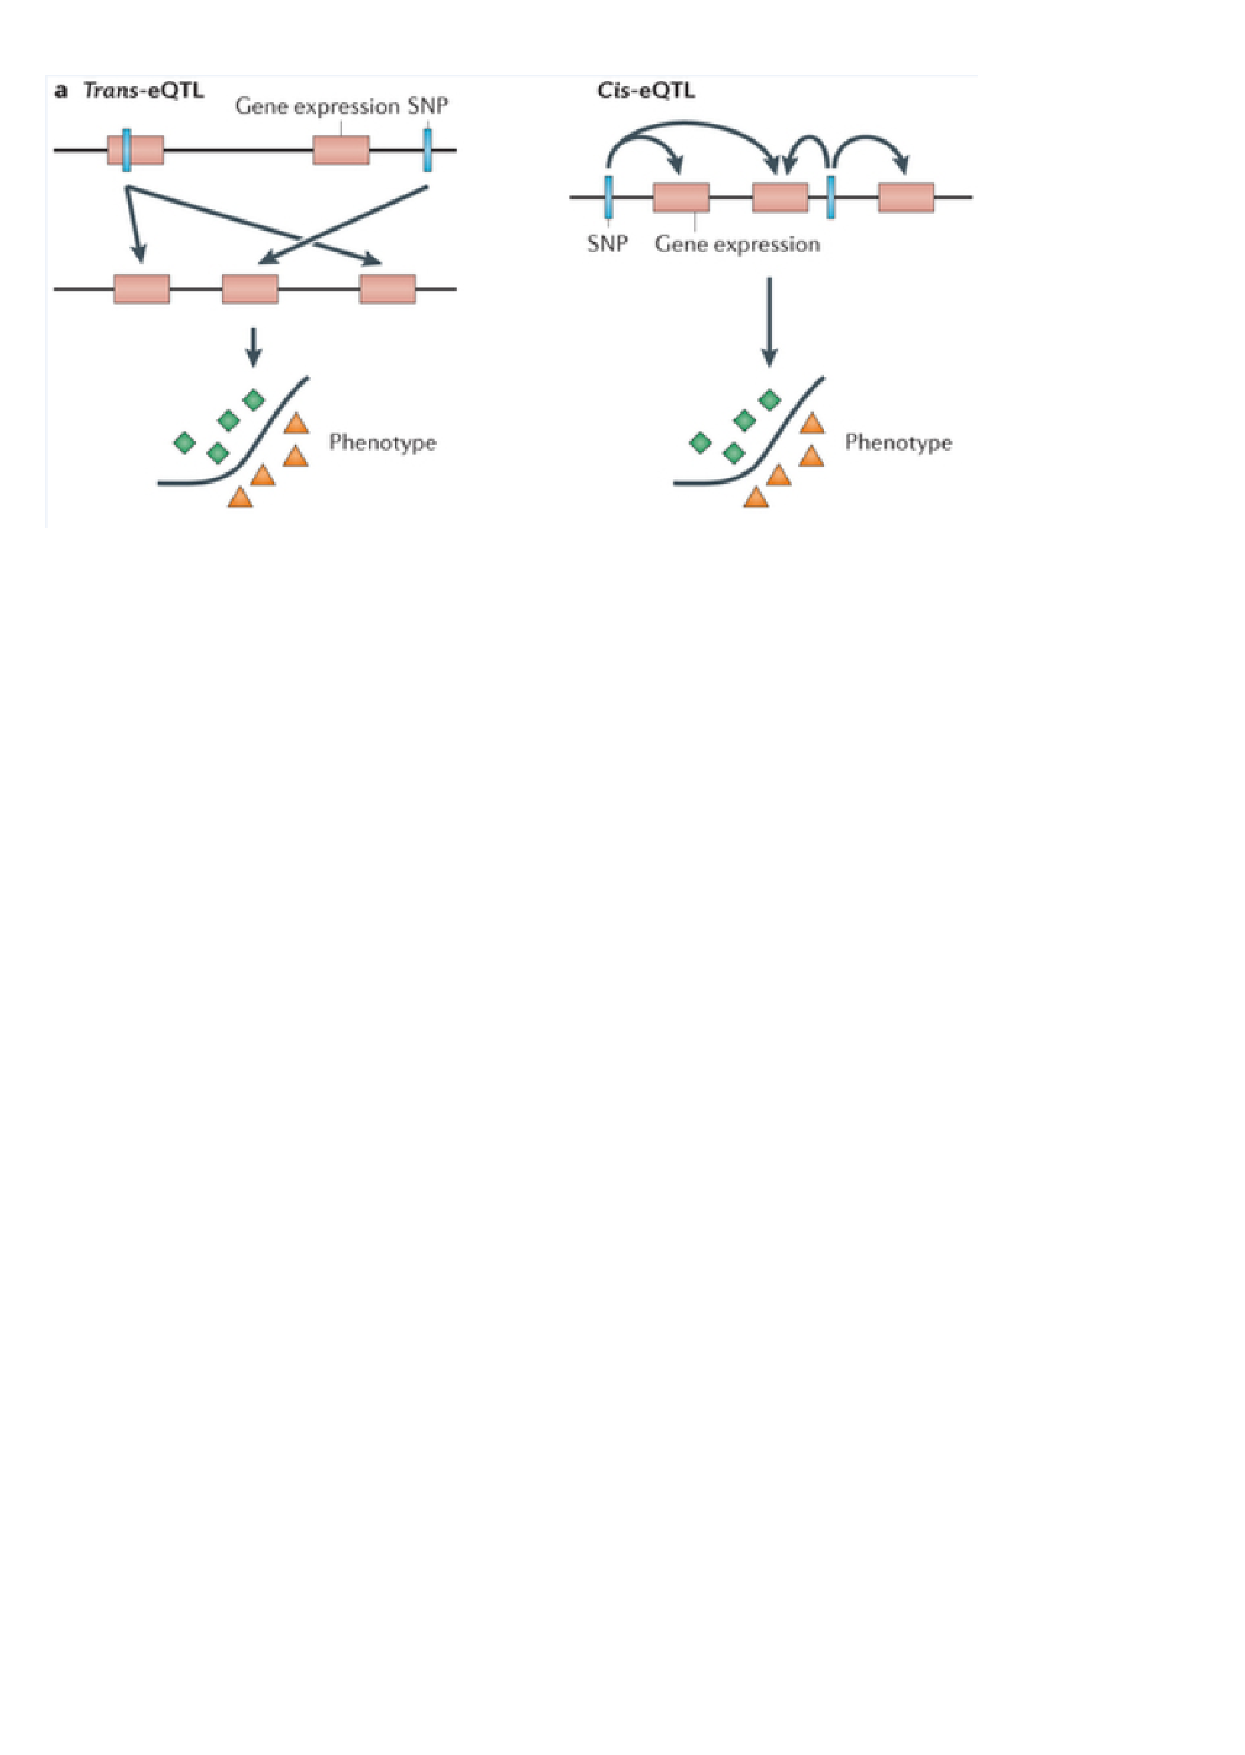
\includegraphics[height=11cm, width=7cm]{figures/multi_staged_1.pdf}} 
  \subfloat[Domain knowledge-guided]{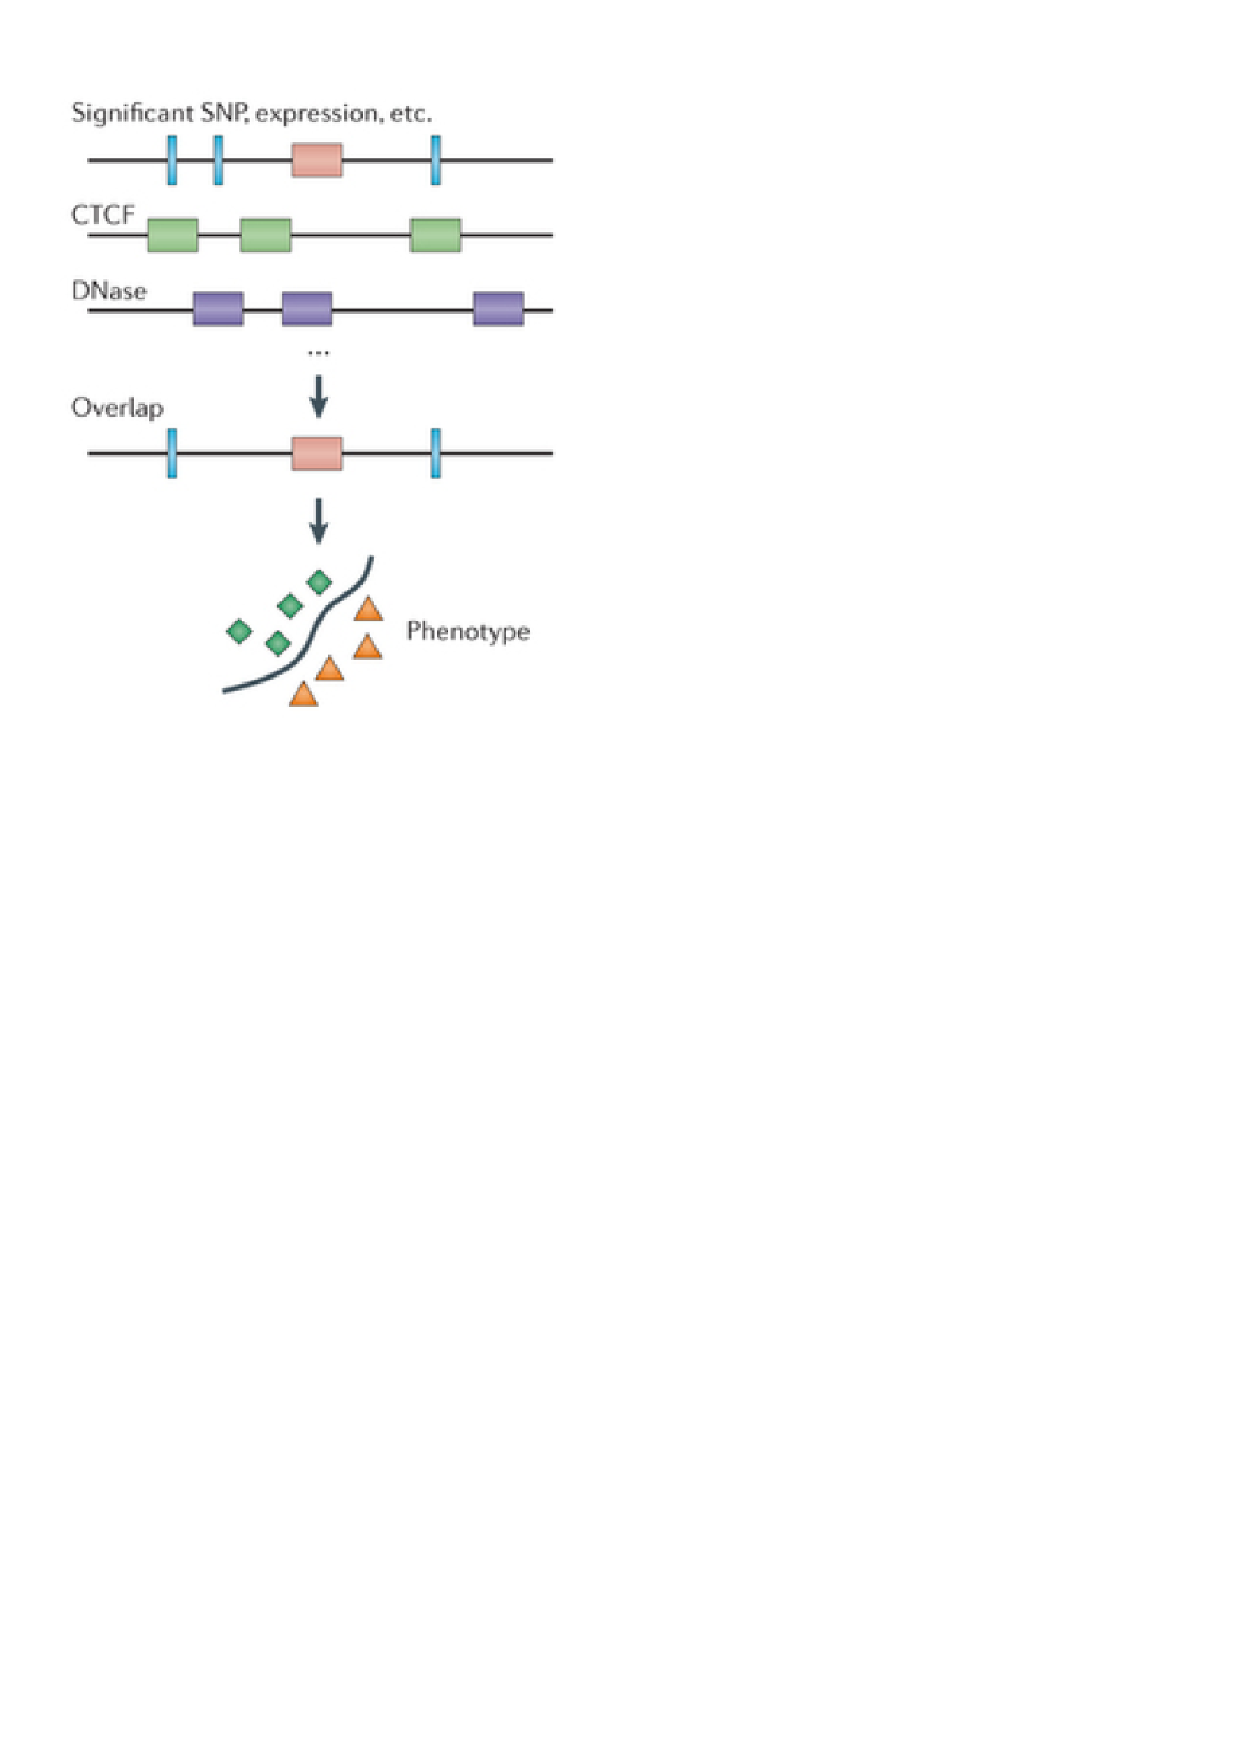
\includegraphics[height=11cm, width=7cm]{figures/multi_staged_2.pdf}}
\end{figure}

\end{frame}


\begin{frame}\frametitle{Genomic variation example}

\begin{figure}
  
\includegraphics[height=10cm, width=8cm]{figures/multi_staged_example_1.pdf}
\end{figure}

\end{frame}


\begin{frame}\frametitle{Genomic variation example}

\begin{figure}
  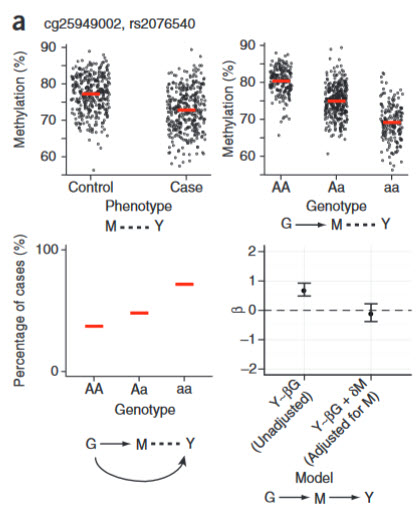
\includegraphics[height=6cm, width=4.5cm]{figures/multi_staged_example_3.jpg}
\end{figure}

\end{frame}


\begin{frame}\frametitle{Genomic variation example}

\begin{itemize}
 \item Mediation analysis
 \item Mendelian randomization (MR)
 \item Conditional Independent test (CIT) 
\end{itemize}

Mediation: \url{https://cran.r-project.org/web/packages/mediation/vignettes/mediation.pdf}
MR: \url{https://cran.r-project.org/web/packages/MendelianRandomization/vignettes/Vignette_MR.pdf}
CIT:\url{https://cran.r-project.org/web/packages/cit/}

\end{frame}


\begin{frame}\frametitle{Mediation analysis}

\begin{figure}
  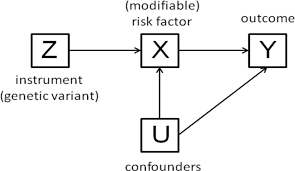
\includegraphics[height=3.5cm, width=6cm]{figures/mendelian_randomization.png}
\end{figure}

See file {\tt mediation.html}

\end{frame}


\begin{frame}\frametitle{Conditional Independent Test}

\begin{figure}
  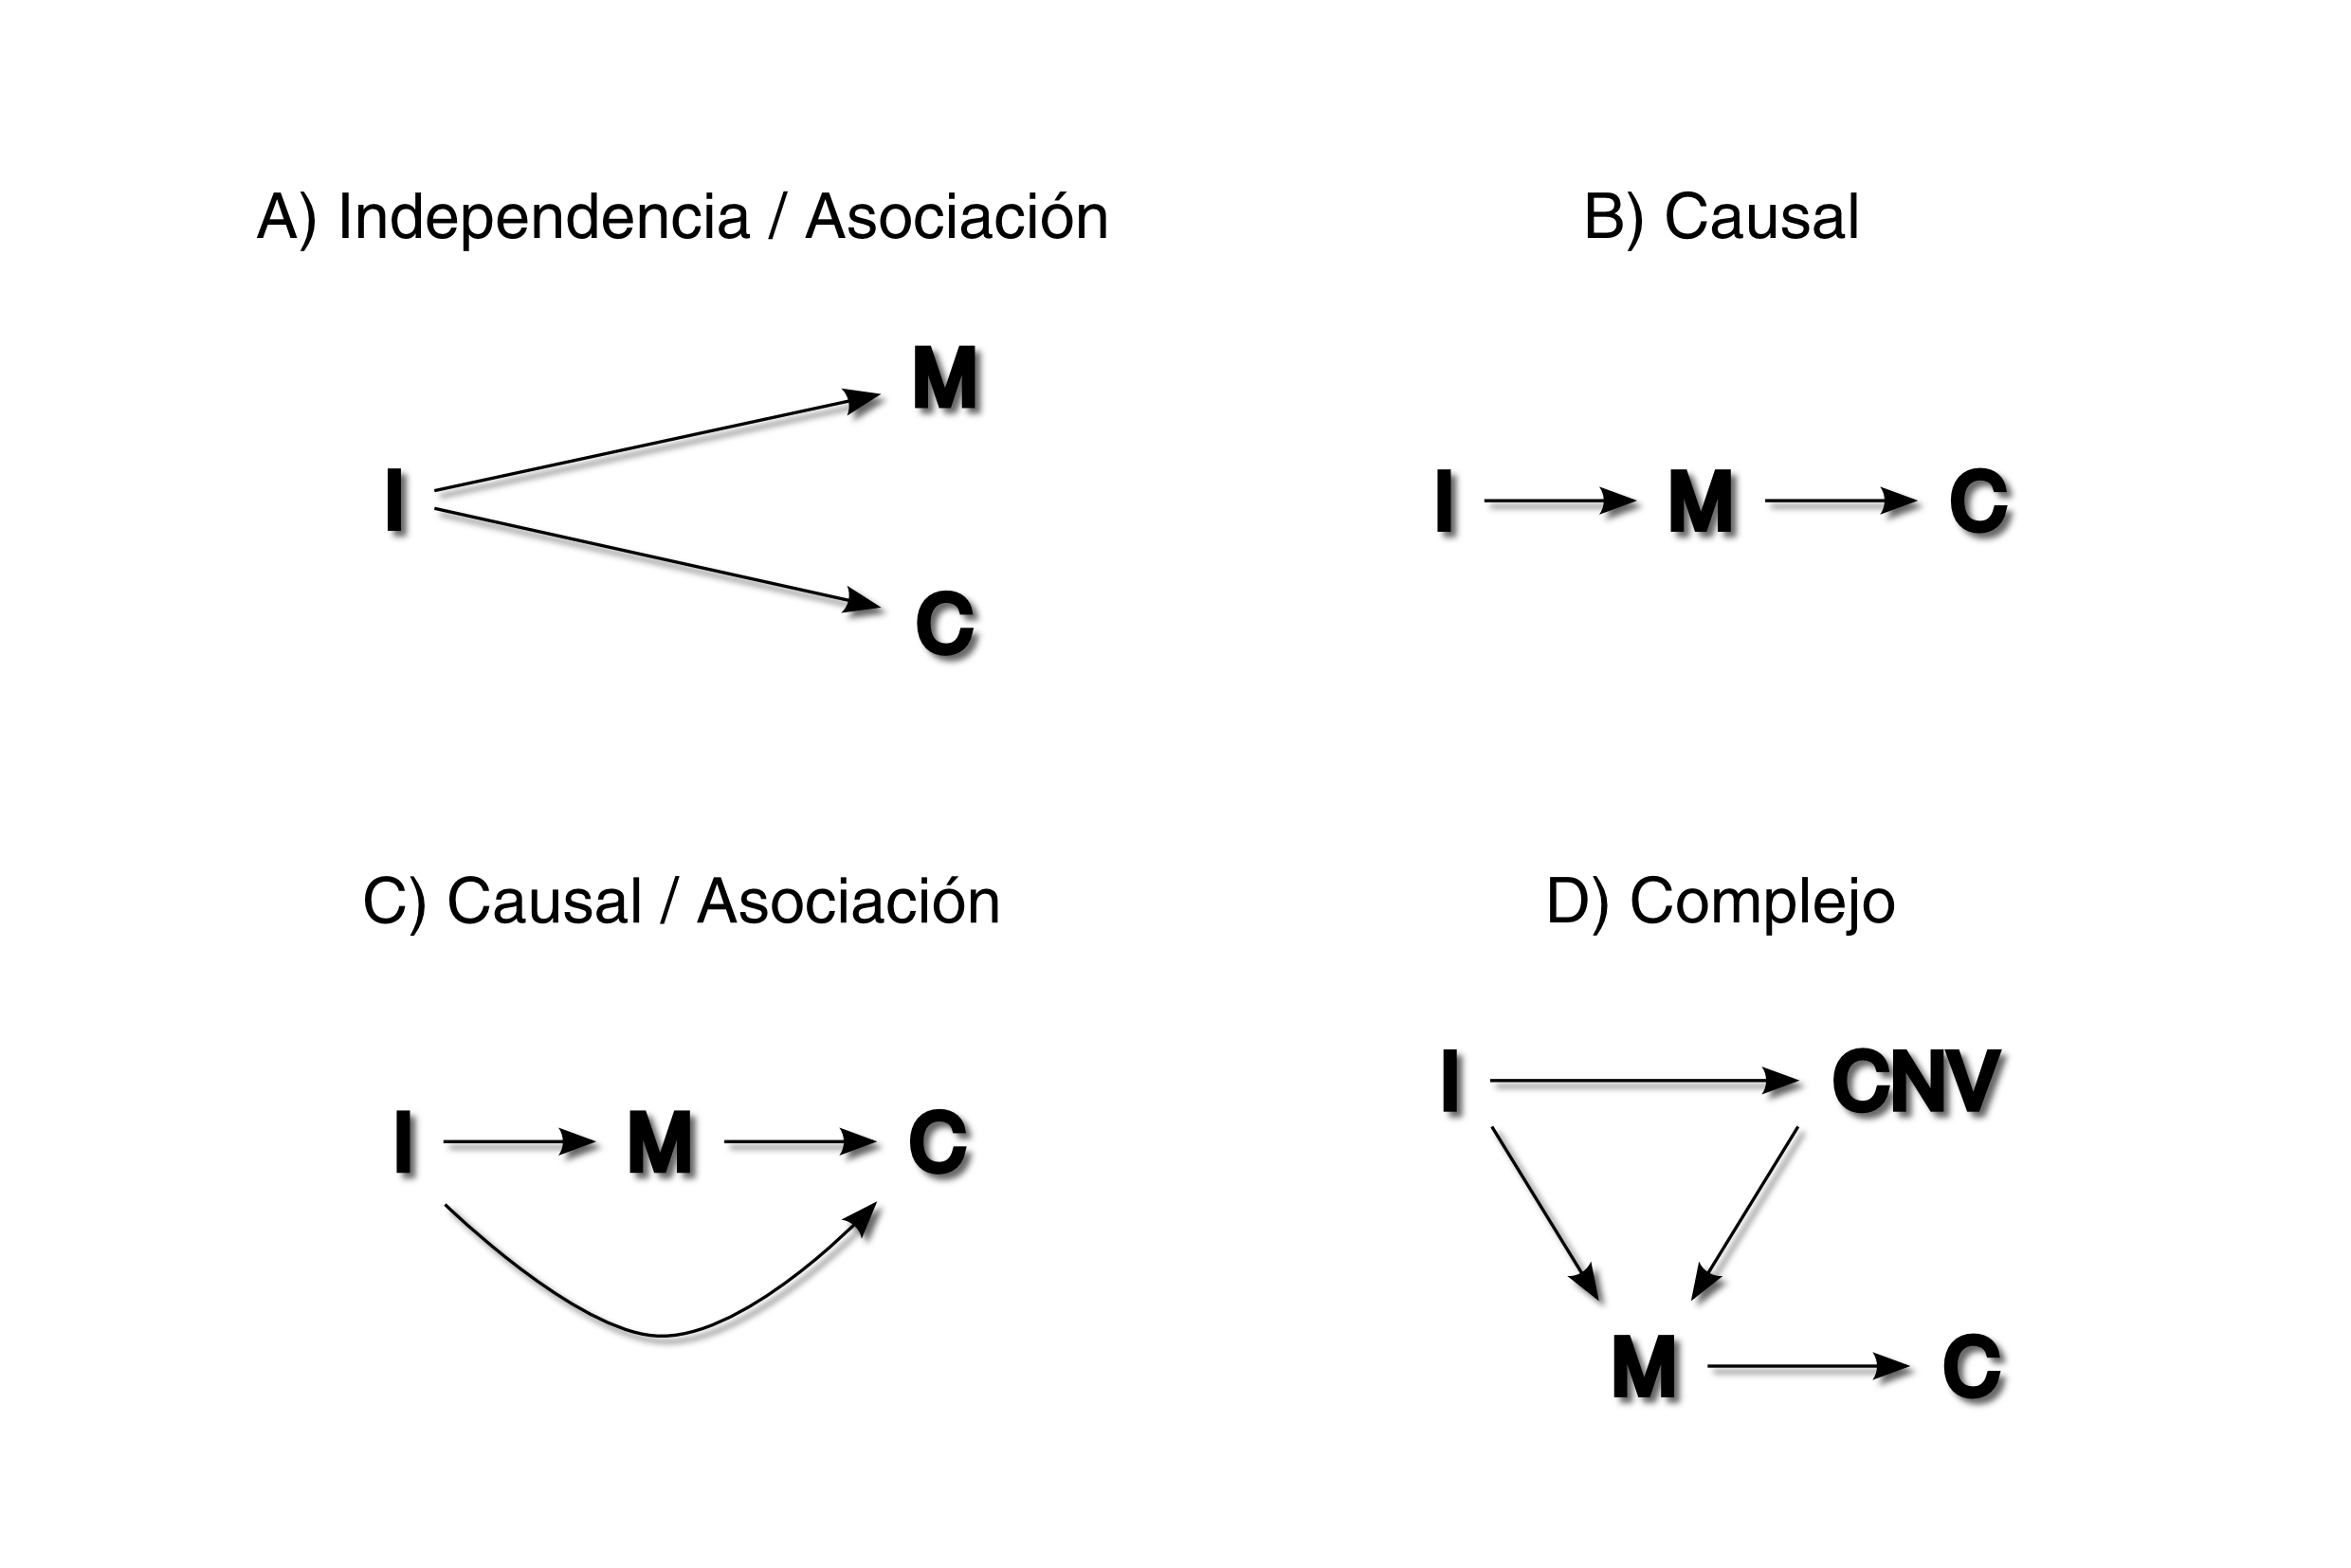
\includegraphics[height=6cm, width=7.5cm]{figures/CIT.png}
\end{figure}

\end{frame}


\begin{frame}\frametitle{Domain knowledge-guided}

\begin{figure}
  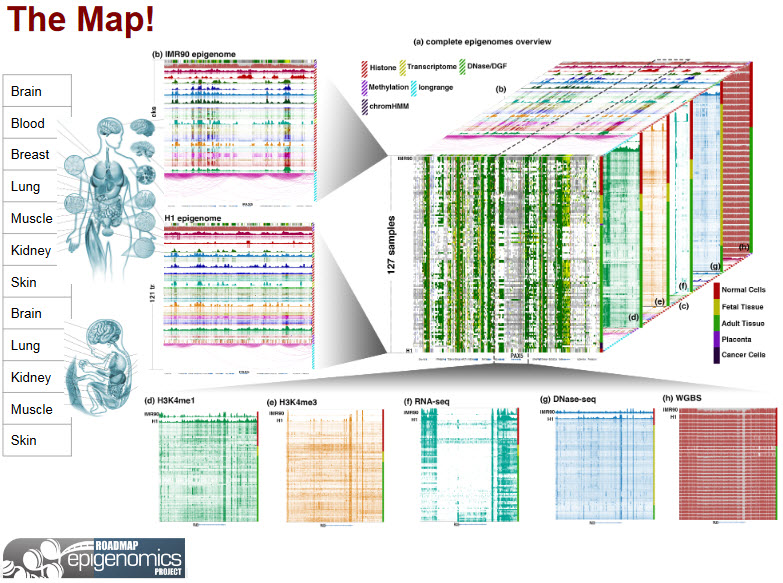
\includegraphics[height=7.5cm, width=6.5cm]{figures/roadmap.jpg}
\end{figure}

\end{frame}




\begin{frame}\frametitle{The RoadMap Epigenomics}

\begin{itemize}
 \item \textcolor{OliveGreen}{Marking of functional genomic elements}
 \item \textcolor{OliveGreen}{Environmental exposures}
 \item Understanding development and differentiation
 \item Regenerative medicine (stem and iPS cells)
 \item Human disease
 \item \textcolor{OliveGreen}{Interpreting GWAS}
 \item Biomarkers, diagnostics and therapies
 \item Exploring cross-talk between epigenomic mechanisms
\end{itemize}

\end{frame}


\begin{frame}\frametitle{Domain knowledge-guided}

\begin{figure}
  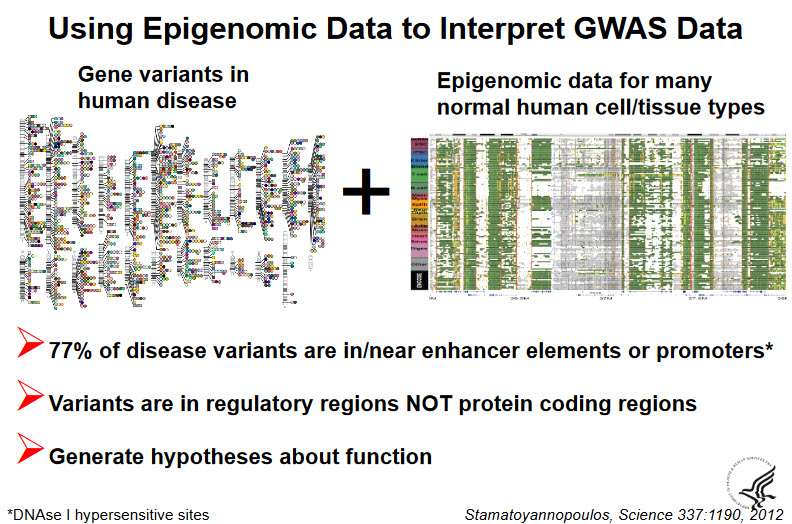
\includegraphics[height=7.5cm, width=6.5cm]{figures/roadmap_utility.jpg}
\end{figure}

\end{frame}



\begin{frame}\frametitle{Domain knowledge-guided}

\begin{figure}
  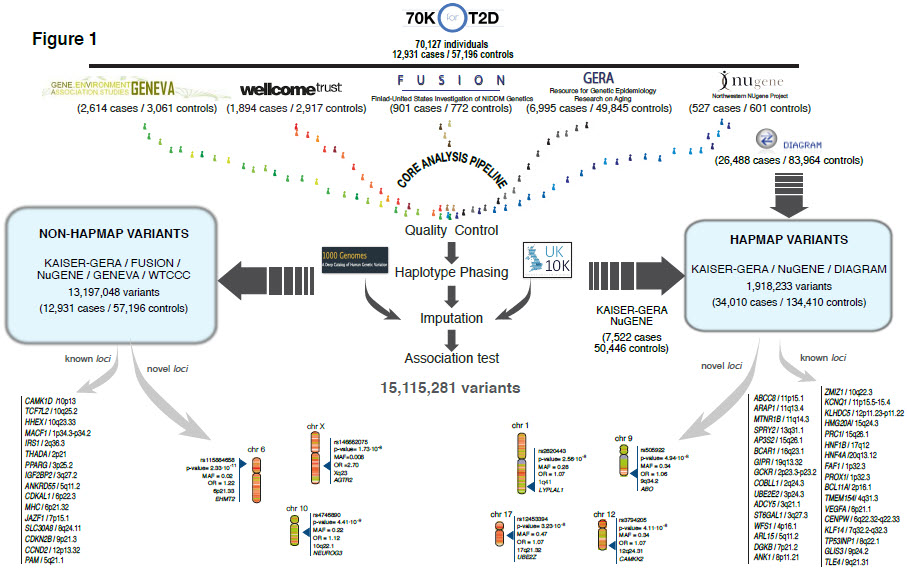
\includegraphics[height=7.5cm, width=6.5cm]{figures/t2d.jpg}
\end{figure}

\end{frame}



\begin{frame}\frametitle{Domain knowledge-guided}

\begin{figure}
  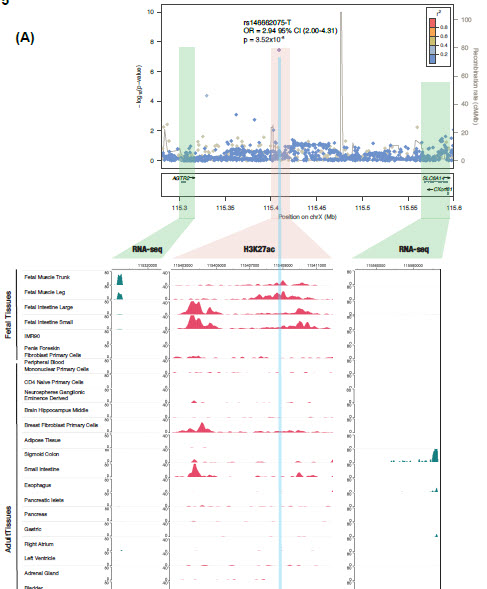
\includegraphics[height=7.5cm, width=6.5cm]{figures/t2d_roadmap.jpg}
\end{figure}

\end{frame}


\begin{frame}[fragile]\frametitle{Domain knowledge-guided}

Let us assume that we want to extract biological information (eQTL, LD, motifs, ...) from large genomic projects such as ENCODE, the 1000 Genomes Project, Roadmap Epigenomics Project and others on the 15 SNPs obtained in paper \textit{Verweij et al. Identification of 15 novel risk loci for coronary artery disease and genetic risk of recurrent events, atrial fibrillation and heart failure. Sci Rep, 7, Article number: 2761 (2017)}. 
\begin{knitrout}\footnotesize
\definecolor{shadecolor}{rgb}{0.969, 0.969, 0.969}\color{fgcolor}\begin{kframe}
\begin{alltt}
\hlkwd{library}\hlstd{(haploR)}
\hlstd{x} \hlkwb{<-} \hlkwd{queryHaploreg}\hlstd{(}\hlkwc{query}\hlstd{=}\hlkwd{c}\hlstd{(}\hlkwd{c}\hlstd{(}\hlstr{"rs11810571"}\hlstd{,} \hlstr{"rs7623687"}\hlstd{,} \hlstr{"rs142695226"}\hlstd{,}
                             \hlstr{"rs433903"}\hlstd{,} \hlstr{"rs10857147"}\hlstd{,} \hlstr{"rs11723436"}\hlstd{,}
                             \hlstr{"rs35879803"}\hlstd{,} \hlstr{"rs35541991"}\hlstd{,} \hlstr{"rs1351525"}\hlstd{,}
                             \hlstr{"rs11170820"}\hlstd{,} \hlstr{"rs2244608"}\hlstd{,} \hlstr{"rs3832966"}\hlstd{,}
                             \hlstr{"rs33928862"}\hlstd{,} \hlstr{"rs7500448"}\hlstd{,} \hlstr{"rs138120077"}\hlstd{)))}
\end{alltt}
\end{kframe}
\end{knitrout}

\end{frame}


\begin{frame}[fragile]\frametitle{Domain knowledge-guided}

We can ask, for instance, information about motifs, gwas, gene name and Enhancer histone marks of those SNPs that are in high LD (>0.9). Notice that the name of all possible variables can shown by typing {\tt names(x)}.

\begin{knitrout}\footnotesize
\definecolor{shadecolor}{rgb}{0.969, 0.969, 0.969}\color{fgcolor}\begin{kframe}
\begin{alltt}
\hlstd{sel} \hlkwb{<-} \hlkwd{as.numeric}\hlstd{(x}\hlopt{$}\hlstd{r2)} \hlopt{>} \hlnum{0.9}
\hlstd{x2} \hlkwb{<-} \hlstd{x[sel,} \hlkwd{c}\hlstd{(}\hlstr{"pos_hg38"}\hlstd{,} \hlstr{"rsID"}\hlstd{,} \hlstr{"Motifs"}\hlstd{,} \hlstr{"gwas"}\hlstd{,}
               \hlstr{"GENCODE_name"}\hlstd{,} \hlstr{"Enhancer_histone_marks"}\hlstd{)]}
\hlstd{x2}
\end{alltt}
\begin{verbatim}
## # A tibble: 258 x 6
##    pos_hg38  rsID       Motifs             gwas  GENCODE_name Enhancer_histone~
##    <fct>     <fct>      <fct>              <fct> <fct>        <fct>            
##  1 75148524  rs10138183 Nanog_disc2        .     TMED10       ""               
##  2 75166305  rs10149880 ERalpha-a_disc2;H~ .     TMED10       ""               
##  3 75139089  rs1047418  Irf_disc5;RBP-Jka~ .     TMED10       ""               
##  4 22606797  rs10485012 AP-4_1;Nkx2_11;Nk~ .     RP1-309H15.2 ""               
##  5 145859799 rs10519748 .                  .     ZNF827       ""               
##  6 151773603 rs1054479  Hoxa13;Pou2f2_kno~ .     TDRKH        ""               
##  7 151788316 rs10788809 Foxj2_1;SP1_disc1  .     TDRKH        ""               
##  8 13266391  rs10832011 Pax-4_1            .     ARNTL        ""               
##  9 13271701  rs10832012 CTCF_disc10;Foxp1  .     ARNTL        ""               
## 10 13273806  rs10832013 DMRT2;HDAC2_disc6~ .     ARNTL        ""               
## # ... with 248 more rows
\end{verbatim}
\end{kframe}
\end{knitrout}

\end{frame}

\begin{frame}[fragile]\frametitle{Domain knowledge-guided}

eQTLs can also be depict by

\begin{knitrout}\footnotesize
\definecolor{shadecolor}{rgb}{0.969, 0.969, 0.969}\color{fgcolor}\begin{kframe}
\begin{alltt}
\hlstd{x3} \hlkwb{<-} \hlstd{x[,} \hlkwd{c}\hlstd{(}\hlstr{"rsID"}\hlstd{,} \hlstr{"eQTL"}\hlstd{)]}
\hlstd{x3}
\end{alltt}
\begin{verbatim}
## # A tibble: 258 x 2
##    rsID       eQTL                                                             
##    <fct>      <fct>                                                            
##  1 rs10138183 GTEx2015_v6,Adipose_Subcutaneous,EIF2B2,3.37702382515779e-19;GTE~
##  2 rs10149880 GTEx2015_v6,Adipose_Subcutaneous,EIF2B2,5.49512183025963e-19;GTE~
##  3 rs1047418  GTEx2015_v6,Adipose_Subcutaneous,EIF2B2,1.19295941493875e-19;GTE~
##  4 rs10485012 .                                                                
##  5 rs10519748 GTEx2015_v6,Artery_Tibial,ZNF827,8.66029894589802e-06            
##  6 rs1054479  GTEx2015_v6,Adipose_Subcutaneous,RP11-98D18.9,2.12743689194852e-~
##  7 rs10788809 GTEx2015_v6,Adipose_Subcutaneous,RP11-98D18.9,1.163639396113e-06~
##  8 rs10832011 GTEx2015_v6,Whole_Blood,ARNTL,1.99939890886288e-10;Lappalainen20~
##  9 rs10832012 GTEx2015_v6,Whole_Blood,ARNTL,8.81903348679608e-09               
## 10 rs10832013 GTEx2015_v6,Whole_Blood,ARNTL,8.8679461832997e-11;Lappalainen201~
## # ... with 248 more rows
\end{verbatim}
\end{kframe}
\end{knitrout}


\end{frame}




%%%%%%%%%%%%%%%%%%%%%%%%%%%%%%
\section{Meta-dimensional analysis}
%%%%%%%%%%%%%%%%%%%%%%%%%%%%%%



\begin{frame}\frametitle{Meta-dimensional analysis}

\begin{itemize}
\item \textcolor{Gray}{Multi-staged analysis: Involves integrating information using a stepwise or hierarchical analysis approach}
\item \textcolor{OliveGreen}{Meta-dimensional analysis}: Refers to the concept of integrating multiple different data types to build a multivariate model associated with a given outcome
\end{itemize}
\end{frame}


\begin{frame}\frametitle{Types of meta-dimensional analyses}

\begin{figure}
\begin{center}
 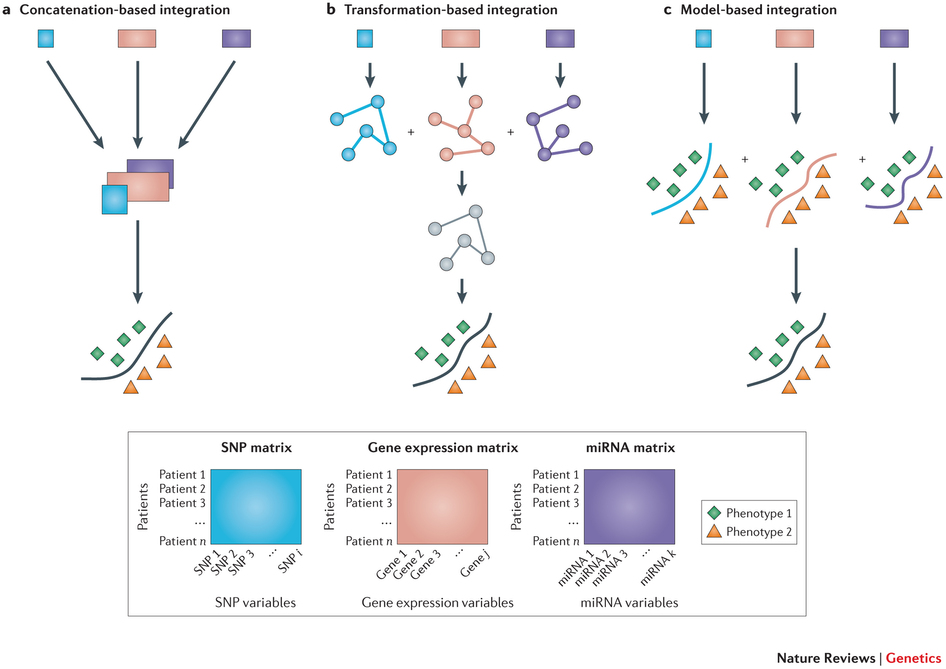
\includegraphics[height=7cm, width=6cm]{figures/meta_dimensional.jpg}
\end{center}
\end{figure}

\end{frame}







%%%%%%%%%%%%%%%%%%%%%%%%%%%%%%%%%%%%%%%%%%%%%%%%%%%%%%%%
\subsection{One omic dataset: dimensionality reduction}
%%%%%%%%%%%%%%%%%%%%%%%%%%%%%%%%%%%%%%%%%%%%%%%%%%%%%%%%



\begin{frame}\frametitle{One omic dataset: dimensionality reduction}

\begin{figure}
\begin{center}
 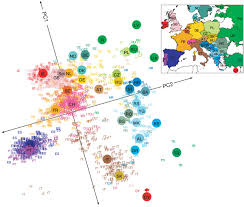
\includegraphics[height=5cm, width=5cm]{figures/pca_example.jpg}
\end{center}
\end{figure}

\end{frame}

\begin{frame}[fragile]\frametitle{One omic dataset: dimensionality reduction}

\begin{itemize}
\item Used to study tissue, cell attributes or cancer signatures with 
regard to abundance of mRNAs, proteins and metabolites
\item Given an omic data set $X$, which is a $n \times p$ matrix, of $n$ individuals and $p$ features
$$ X=(x_1, x_2, \ldots, x_p)$$ 
\item we look for new variables that are linear combinations of the original variables
$f=q_1X_1 + q_2X_2 + \ldots + q_pX_p$  or $f=Xq$ where $q$ are know as loadings.
\item We introduce the restriction that for $i$th component, $q$'s should maximize the variance components of $f$'s
$$ \argmax_{q^i} \text{var}(Xq^i)$$ and $q$'s has to be orthogonal to each other.
\end{itemize}

\end{frame}

\begin{frame}[fragile]\frametitle{One omic dataset: dimensionality reduction}

\begin{knitrout}\footnotesize
\definecolor{shadecolor}{rgb}{0.969, 0.969, 0.969}\color{fgcolor}

{\centering 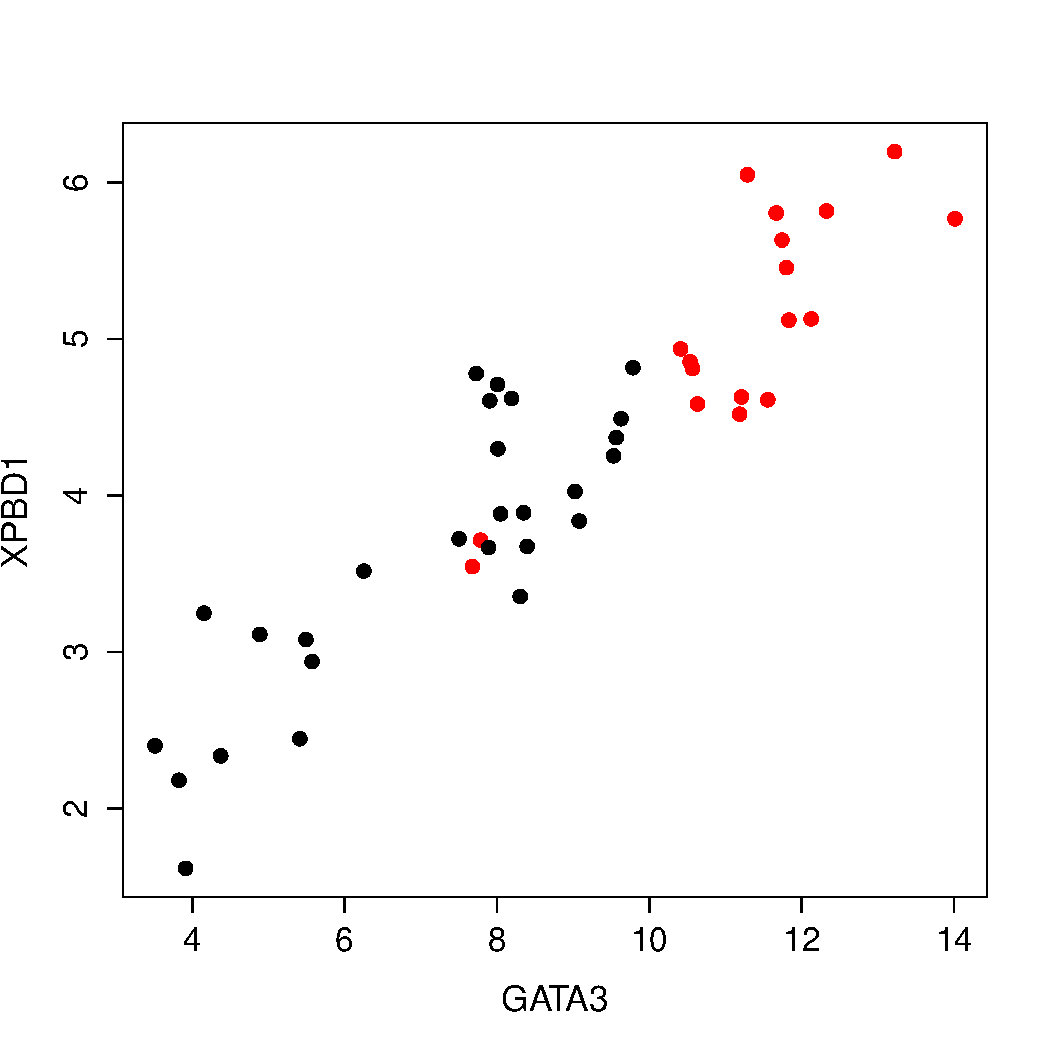
\includegraphics[width=2in]{figure/plot_pca_1-1} 

}



\end{knitrout}

\end{frame}

\begin{frame}[fragile]\frametitle{One omic dataset: dimensionality reduction}

\begin{knitrout}\footnotesize
\definecolor{shadecolor}{rgb}{0.969, 0.969, 0.969}\color{fgcolor}

{\centering 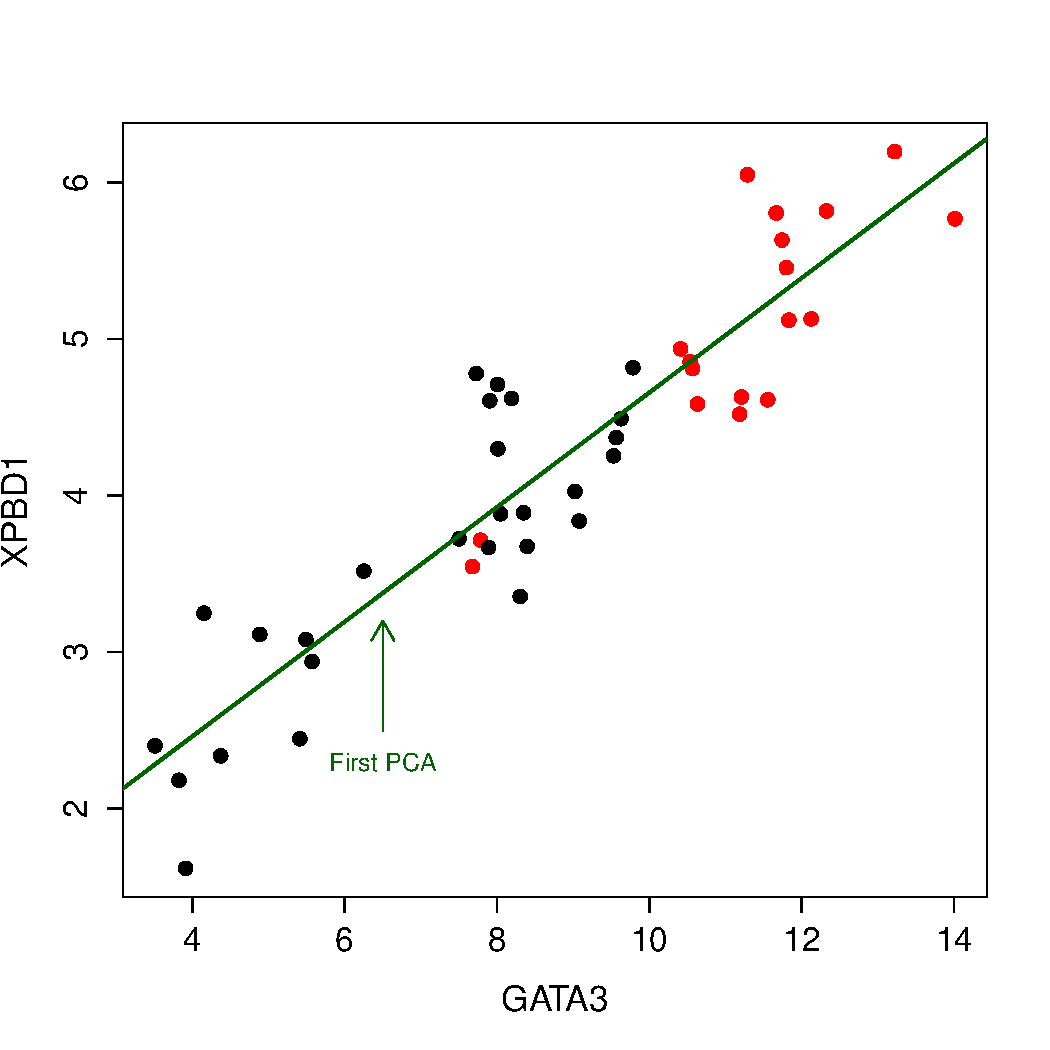
\includegraphics[width=2in]{figure/plot_pca_2-1} 

}



\end{knitrout}

\end{frame}


\begin{frame}[fragile]\frametitle{One omic dataset: dimensionality reduction}

\begin{knitrout}\footnotesize
\definecolor{shadecolor}{rgb}{0.969, 0.969, 0.969}\color{fgcolor}

{\centering 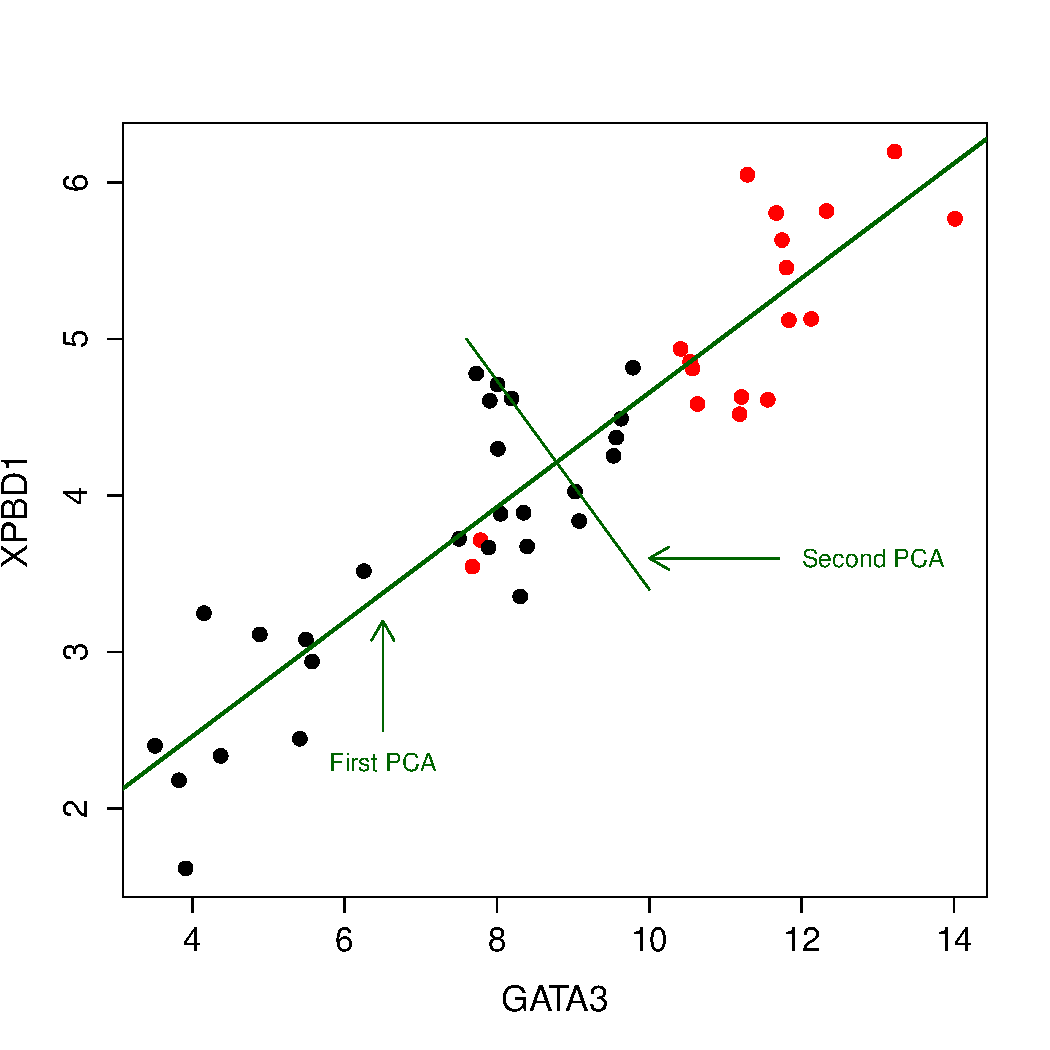
\includegraphics[width=2in]{figure/plot_pca_3-1} 

}



\end{knitrout}

\end{frame}




\begin{frame}[fragile]\frametitle{One omic dataset: dimensionality reduction}

\begin{knitrout}\footnotesize
\definecolor{shadecolor}{rgb}{0.969, 0.969, 0.969}\color{fgcolor}

{\centering 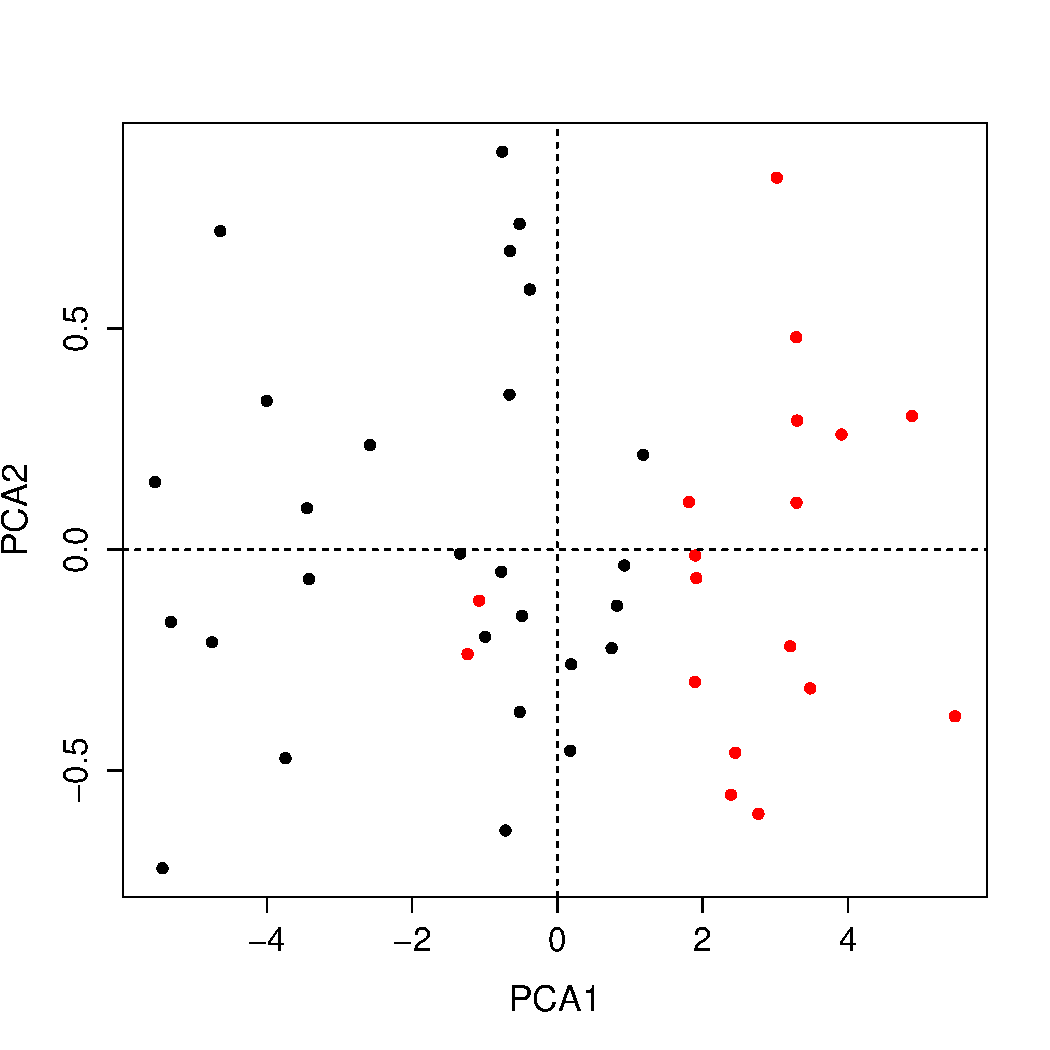
\includegraphics[width=2in]{figure/plot_pca_4-1} 

}



\end{knitrout}

\end{frame}


\begin{frame}[fragile]\frametitle{One omic dataset: dimensionality reduction}

Data visualization: biplot

\begin{knitrout}\footnotesize
\definecolor{shadecolor}{rgb}{0.969, 0.969, 0.969}\color{fgcolor}

{\centering 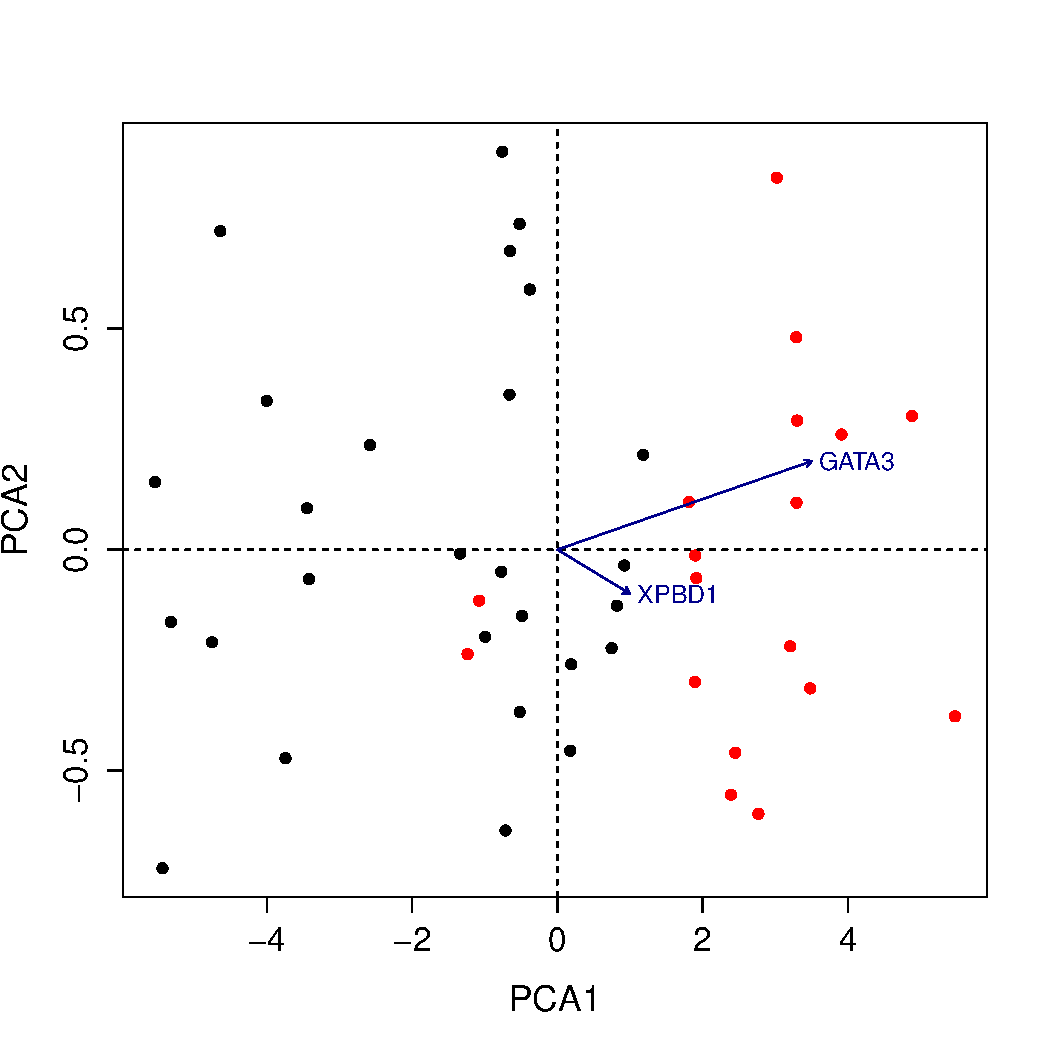
\includegraphics[width=2in]{figure/plot_pca_5-1} 

}



\end{knitrout}

\end{frame}


\begin{frame}[fragile]\frametitle{One omic dataset: dimensionality reduction}

\begin{itemize}
\item There are other thechniques such as: Principal co-ordinate analysis (PCoA), correspondence analysis (CA) and nonsymetrical correspondence analysis (NSCA).
\pause
\item They can be applied to other types of data (e.g. non-continuous). PCoA can also be applied to binary or count data.
\pause
\item PCA is designed to analyze multi-normal distributed data. If data are skweed, contain extreme outliers, or display nonlinear trends, other methods such as 
Multidimendional Scaling (MDS)
\pause
\item Nonnegative matrix factorization (NMF) and Independent Component Analysis (ICA) are applied when orthogonality or independence acrross components are not hold.
\end{itemize}

\end{frame}


\begin{frame}[fragile]\frametitle{One omic dataset: dimensionality reduction}

 \begin{itemize}
 \item Solving the problem for the $i$-th component $$ \argmax_{q^i} \text{var}(Xq^i)$$ uses SVD decomposition and it requires and inversion step that can be problematic when   $p >> n$
 \item Several extensions based on reguralization step or L-1 penalization (Least Absolute Shrinkage and Selection Operator, LASSO) can be applied
 \item Sparse, penalized and reguralized extensions of PCA and related method have been proposed in omic data analysis, recently (sPCA)
 \end{itemize}
\end{frame}



\begin{frame}{Multi-omic real data}

\begin{itemize}
  \item Data from the Cancer Genome Atlas (TCGA) will be analyzed.
  \item A subset of the TCGA breast cancer study from Nature 2012 publication have been selected.
  \item Data {\tt https://tcga-data.nci.nih.gov/docs/publications/brca\_2012/}.
  \item Available data are: miRNA, miRNAprecursor, RNAseq, Methylation, proteins from a RPPA array, and  GISTIC SNP calls (CNA and LOH). Clinical data are also available.
 \end{itemize}

\end{frame}


\begin{frame}[fragile]\frametitle{Multi-omic real data}

Data can be loaded into {\tt R} by executing:

\begin{knitrout}\footnotesize
\definecolor{shadecolor}{rgb}{0.969, 0.969, 0.969}\color{fgcolor}\begin{kframe}
\begin{alltt}
\hlkwd{load}\hlstd{(}\hlstr{"data/breast_TCGA_subset_multi_omic.RData"}\hlstd{)}
\hlkwd{summary}\hlstd{(breast_multi)}
\end{alltt}
\begin{verbatim}
##                Length Class      Mode   
## miRNA              79 data.frame list   
## miRNAprecursor     79 data.frame list   
## RNAseq         791580 -none-     numeric
## Methyl             79 data.frame list   
## RPPA               79 data.frame list   
## LOH            996348 -none-     numeric
## CNA            934649 -none-     numeric
## clin               29 data.frame list
\end{verbatim}
\end{kframe}
\end{knitrout}
\end{frame}



\begin{frame}[fragile]\frametitle{PCA analysis}

\begin{knitrout}\footnotesize
\definecolor{shadecolor}{rgb}{0.969, 0.969, 0.969}\color{fgcolor}\begin{kframe}
\begin{alltt}
\hlkwd{require}\hlstd{(ade4)}
\hlkwd{dim}\hlstd{(breast_multi}\hlopt{$}\hlstd{RNAseq)}
\end{alltt}
\begin{verbatim}
## [1] 10020    79
\end{verbatim}
\end{kframe}
\end{knitrout}

\begin{knitrout}\footnotesize
\definecolor{shadecolor}{rgb}{0.969, 0.969, 0.969}\color{fgcolor}\begin{kframe}
\begin{alltt}
\hlstd{breastPCA}\hlkwb{<-}\hlkwd{dudi.pca}\hlstd{(breast_multi}\hlopt{$}\hlstd{RNAseq,}
            \hlkwc{scannf}\hlstd{=}\hlnum{FALSE}\hlstd{,} \hlkwc{nf}\hlstd{=}\hlnum{5}\hlstd{)}
\end{alltt}
\end{kframe}
\end{knitrout}
\end{frame}


\begin{frame}[fragile]\frametitle{PCA analysis}

There is a BioC package called made4 which is a wrapper oround ade4 that 
utilizes Bioconductor data classes (such as {\tt Expression Set} to help 
visualizing the results). They key function ir {\tt ord}. The panels shows
plot of eignevalues, projections of samples, projections of genes and biplot.

\begin{knitrout}\footnotesize
\definecolor{shadecolor}{rgb}{0.969, 0.969, 0.969}\color{fgcolor}\begin{kframe}
\begin{alltt}
\hlkwd{require}\hlstd{(made4)}
\end{alltt}
\end{kframe}
\end{knitrout}

\begin{knitrout}\footnotesize
\definecolor{shadecolor}{rgb}{0.969, 0.969, 0.969}\color{fgcolor}\begin{kframe}
\begin{alltt}
\hlstd{group}\hlkwb{<-}\hlkwd{droplevels}\hlstd{(breast_multi}\hlopt{$}\hlstd{clin}\hlopt{$}\hlstd{ER.Status)}
\hlstd{out} \hlkwb{<-} \hlkwd{ord}\hlstd{(breast_multi}\hlopt{$}\hlstd{RNAseq,} \hlkwc{classvec}\hlstd{=group)}
\hlkwd{plot}\hlstd{(out,} \hlkwc{nlab}\hlstd{=}\hlnum{3}\hlstd{,} \hlkwc{arraylabels}\hlstd{=}\hlkwd{rep}\hlstd{(}\hlstr{"T"}\hlstd{,} \hlnum{79}\hlstd{))}
\end{alltt}
\end{kframe}
\end{knitrout}
\end{frame}


\begin{frame}[fragile]\frametitle{PCA analysis}

\begin{figure}
\begin{center}
 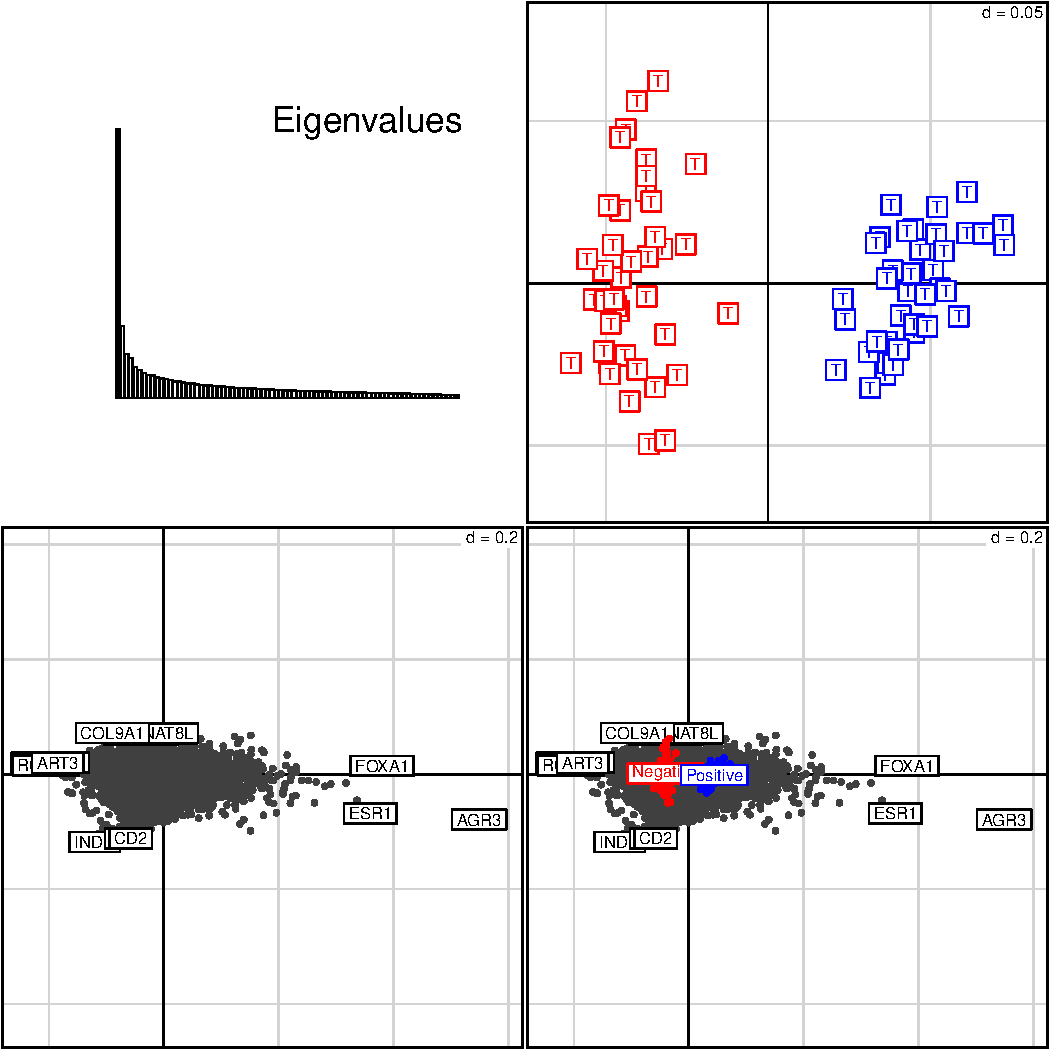
\includegraphics[width=5.5cm]{figure/pca_plot-1}
\end{center}
\end{figure}
\end{frame}

\begin{frame}[fragile]\frametitle{PCA analysis}

Sample and genes projections can also be plotted using another wrapper around
{\tt ade4} package. By default the top-10 more important genes for each axis
are highlighted.
\begin{knitrout}\footnotesize
\definecolor{shadecolor}{rgb}{0.969, 0.969, 0.969}\color{fgcolor}\begin{kframe}
\begin{alltt}
\hlkwd{par}\hlstd{(}\hlkwc{mfrow}\hlstd{=}\hlkwd{c}\hlstd{(}\hlnum{2}\hlstd{,}\hlnum{1}\hlstd{))}
\hlkwd{plotarrays}\hlstd{(out}\hlopt{$}\hlstd{ord}\hlopt{$}\hlstd{co,} \hlkwc{classvec}\hlstd{=group)}
\hlkwd{plotgenes}\hlstd{(out,} \hlkwc{col}\hlstd{=}\hlstr{"blue"}\hlstd{)}
\end{alltt}
\end{kframe}
\end{knitrout}
\end{frame}


\begin{frame}[fragile]\frametitle{PCA analysis}

\begin{figure}
\begin{center}
 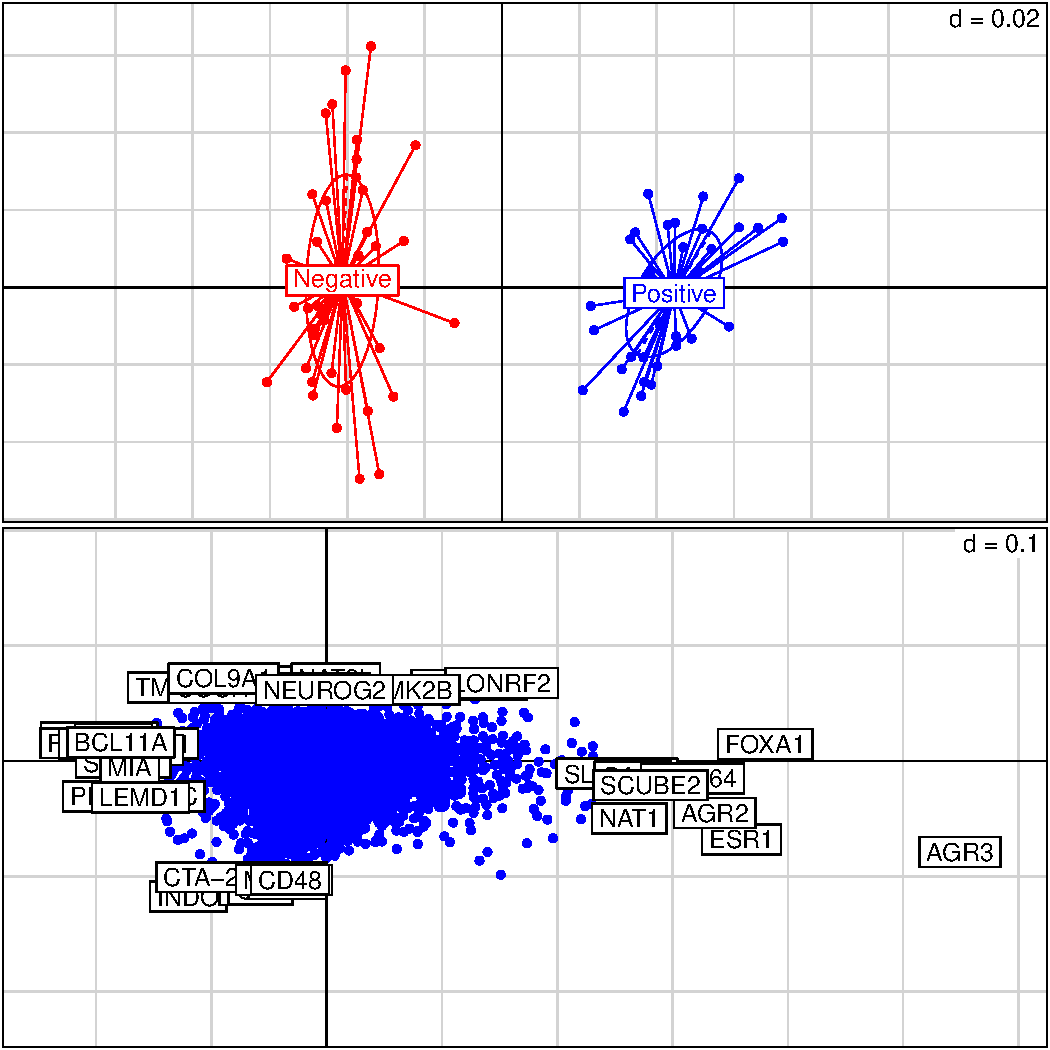
\includegraphics[width=5.5cm]{figure/projections_plot-1}
\end{center}
\end{figure}


\end{frame}


\begin{frame}[fragile]\frametitle{PCA analysis}

A list of variables with higher loadings on axes can be obtained using the following
function

\begin{knitrout}\footnotesize
\definecolor{shadecolor}{rgb}{0.969, 0.969, 0.969}\color{fgcolor}\begin{kframe}
\begin{alltt}
\hlstd{ax1} \hlkwb{<-} \hlkwd{topgenes}\hlstd{(out,} \hlkwc{axis}\hlstd{=}\hlnum{1}\hlstd{,} \hlkwc{n}\hlstd{=}\hlnum{5}\hlstd{)}
\hlstd{ax2} \hlkwb{<-} \hlkwd{topgenes}\hlstd{(out,} \hlkwc{axis}\hlstd{=}\hlnum{2}\hlstd{,} \hlkwc{n}\hlstd{=}\hlnum{5}\hlstd{)}
\hlkwd{cbind}\hlstd{(ax1, ax2)}
\end{alltt}
\begin{verbatim}
##       ax1       ax2      
##  [1,] "ROPN1B"  "SH3GL2" 
##  [2,] "ROPN1"   "SLITRK6"
##  [3,] "FOXA1"   "LONRF2" 
##  [4,] "SFRP1"   "IL7R"   
##  [5,] "ESR1"    "INDO"   
##  [6,] "AGR3"    "NAT8L"  
##  [7,] "AGR2"    "UBD"    
##  [8,] "C1orf64" "CD2"    
##  [9,] "ART3"    "CD69"   
## [10,] "BCL11A"  "COL9A1"
\end{verbatim}
\end{kframe}
\end{knitrout}

\end{frame}



\begin{frame}[fragile]\frametitle{Sparse PCA analysis}

Witten D, Tibshirani R, Hastie T (Biostatistics, 2009, 10(3):515-534) presented a penalized matrix decomposition for computing a rank-K approximation for a matrix based on L1-penalization. The method is also extended to Canonical Correlation Analysis (CCA).

\begin{knitrout}\footnotesize
\definecolor{shadecolor}{rgb}{0.969, 0.969, 0.969}\color{fgcolor}\begin{kframe}
\begin{alltt}
\hlkwd{require}\hlstd{(PMA)}
\hlstd{dd} \hlkwb{<-} \hlkwd{t}\hlstd{(breast_multi}\hlopt{$}\hlstd{RNAseq)}
\hlstd{sout} \hlkwb{<-} \hlkwd{SPC}\hlstd{(dd,} \hlkwc{sumabsv}\hlstd{=}\hlnum{3}\hlstd{,}
            \hlkwc{K}\hlstd{=}\hlnum{2}\hlstd{,} \hlkwc{orth}\hlstd{=}\hlnum{TRUE}\hlstd{)}
\end{alltt}
\begin{verbatim}
## 12345678910
## 1234567891011121314151617181920
\end{verbatim}
\end{kframe}
\end{knitrout}

NOTE: {\tt subabsv} argument controls the degree of sparsity. It can be tuned by using {\tt SPC.cv} function

\end{frame}


\begin{frame}[fragile]\frametitle{Sparse PCA analysis}

\begin{knitrout}\scriptsize
\definecolor{shadecolor}{rgb}{0.969, 0.969, 0.969}\color{fgcolor}\begin{kframe}
\begin{alltt}
\hlkwd{rownames}\hlstd{(sout}\hlopt{$}\hlstd{u)} \hlkwb{<-} \hlkwd{rownames}\hlstd{(dd)}
\hlkwd{rownames}\hlstd{(sout}\hlopt{$}\hlstd{v)} \hlkwb{<-} \hlkwd{colnames}\hlstd{(dd)}
\hlkwd{head}\hlstd{(sout}\hlopt{$}\hlstd{u)}
\end{alltt}
\begin{verbatim}
##                    [,1]       [,2]
## TCGA-C8-A12V -0.1266630 -0.2198702
## TCGA-A2-A0ST -0.1052587 -0.2464092
## TCGA-E2-A159 -0.1057203 -0.1662398
## TCGA-BH-A0BW -0.1335251 -0.1229296
## TCGA-A2-A0SX -0.1520058 -0.1327320
## TCGA-AR-A1AI -0.1768082 -0.1491056
\end{verbatim}
\begin{alltt}
\hlkwd{head}\hlstd{(sout}\hlopt{$}\hlstd{v)}
\end{alltt}
\begin{verbatim}
##          [,1] [,2]
## CREB3L1     0    0
## PNMA1       0    0
## MMP2        0    0
## C10orf90    0    0
## GPR98       0    0
## APBB2       0    0
\end{verbatim}
\end{kframe}
\end{knitrout}

\end{frame}

\begin{frame}[fragile]\frametitle{Sparse PCA analysis}

\begin{knitrout}\footnotesize
\definecolor{shadecolor}{rgb}{0.969, 0.969, 0.969}\color{fgcolor}\begin{kframe}
\begin{alltt}
\hlkwd{plot}\hlstd{(sout}\hlopt{$}\hlstd{u,} \hlkwc{type}\hlstd{=}\hlstr{"n"}\hlstd{,} \hlkwc{xlab}\hlstd{=}\hlstr{"First sPCA"}\hlstd{,} \hlkwc{ylab}\hlstd{=}\hlstr{"Second sPCA"}\hlstd{)}
\hlkwd{points}\hlstd{(sout}\hlopt{$}\hlstd{u,} \hlkwc{col}\hlstd{=}\hlkwd{as.numeric}\hlstd{(group))}
\end{alltt}
\end{kframe}

{\centering 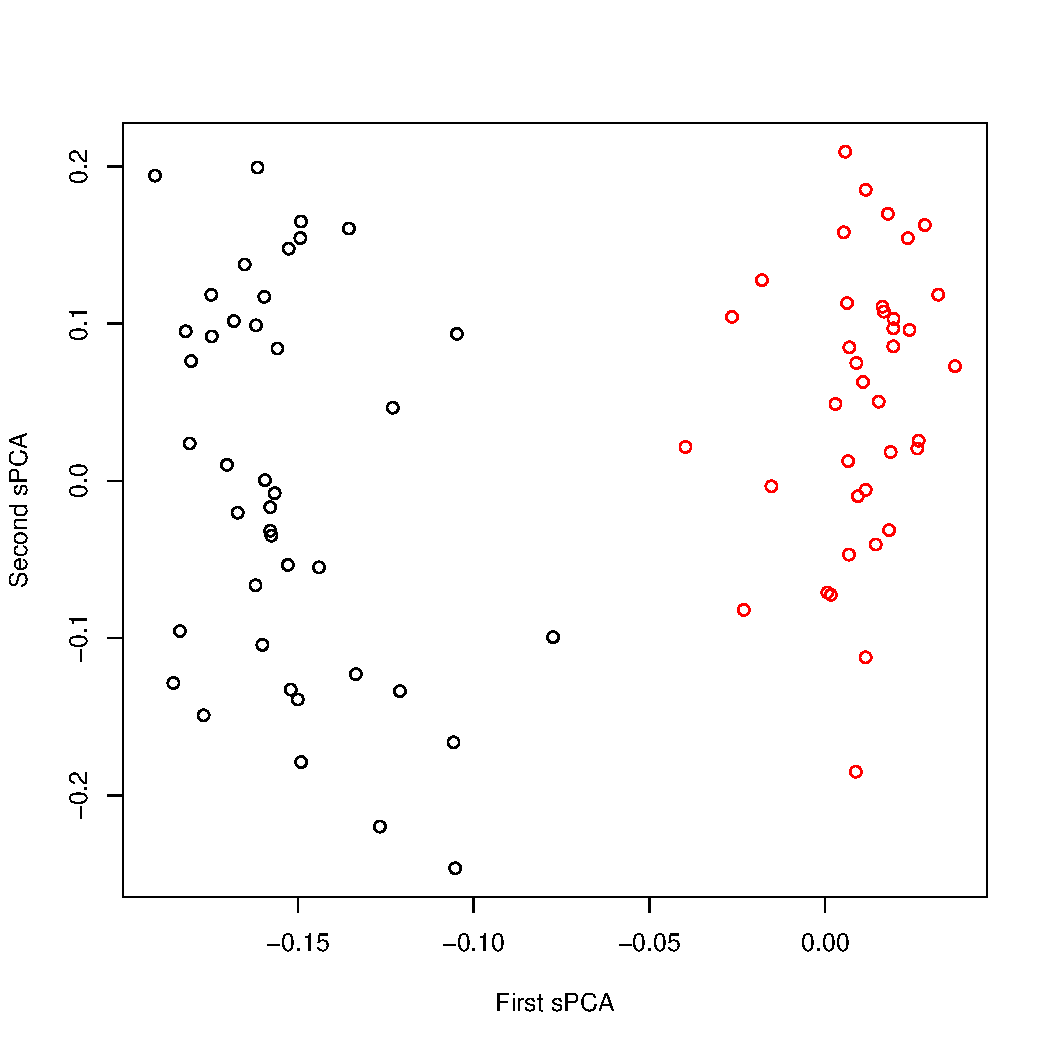
\includegraphics[width=2in]{figure/sPCA_plot-1} 

}



\end{knitrout}

\end{frame}


\begin{frame}[fragile]\frametitle{Sparse PCA analysis}

\begin{knitrout}\scriptsize
\definecolor{shadecolor}{rgb}{0.969, 0.969, 0.969}\color{fgcolor}\begin{kframe}
\begin{alltt}
\hlstd{ss} \hlkwb{<-} \hlstd{sout}\hlopt{$}\hlstd{v[,}\hlnum{1}\hlstd{]}
\hlstd{ss[ss}\hlopt{!=}\hlnum{0}\hlstd{]}
\end{alltt}
\begin{verbatim}
##       FSIP1      ROPN1B     SLC44A4       ROPN1       FOXA1     SCGB2A2 
##  0.12976786 -0.20047758  0.09854402 -0.22180706  0.35283734  0.02914304 
##        CA12     HORMAD1        TFF3      ABCC11        ESR1        AGR3 
##  0.08389962 -0.11978720  0.01092539  0.01843790  0.26810418  0.69491639 
##        AGR2     C1orf64      SCUBE2        ART3 
##  0.29917578  0.23368898  0.05023190 -0.18825577
\end{verbatim}
\begin{alltt}
\hlstd{ax1}
\end{alltt}
\begin{verbatim}
##  [1] "ROPN1B"  "ROPN1"   "FOXA1"   "SFRP1"   "ESR1"    "AGR3"    "AGR2"   
##  [8] "C1orf64" "ART3"    "BCL11A"
\end{verbatim}
\end{kframe}
\end{knitrout}

\end{frame}



%%%%%%%%%%%%%%%%%%%%%%%%%%%%%%%%%%%
\subsection{Integrating two or more omic datasets}
%%%%%%%%%%%%%%%%%%%%%%%%%%%%%%%%%%%



\begin{frame}\frametitle{One omic dataset: dimensionality reduction}

\begin{figure}
\begin{center}
 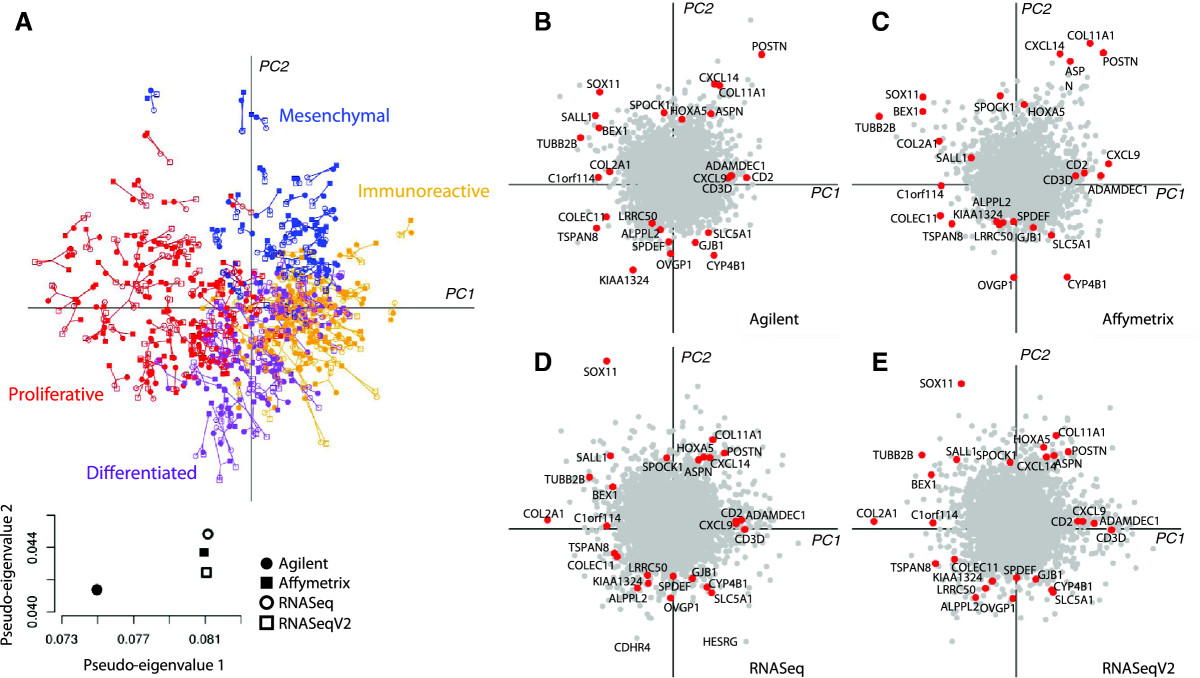
\includegraphics[height=5.5cm, width=6cm]{figures/multi_example.jpg}
\end{center}
\end{figure}

\end{frame}


\begin{frame}\frametitle{Integrating two or more omic datasets}

\begin{itemize}
\item There are methods based on dimension reduction techniques: generalized SVD, Co-Inertia Analysis (CIA), sparse or penalized extensions of Partial Least Squares (PLS),
Canonical Correlation (CCA), Multiple Factor Analysis (MFA), Generalized Canonical Correlation (GCA)
\pause
\item There are methods that are based on path modelling: structural equation models (SEM)
\pause
\item Reguralized Generalized Canonical Correlation (RGCA) provides a unified framework for different approaches (Tenenhaus, M. and Tenenhaus, A. Psychometrika, 2011, 76(2):257-284). Other methods are special cases of RGCA.
\pause
\item RGCA integrates a feature selection method, named sparse GCCA (SGCCA) (Tenenhaus, A et al. Biostatistics, 2014, 15(3):569-83).
\end{itemize}

\end{frame}




\begin{frame}\frametitle{Integrating two or more omic datasets}

\begin{itemize}
\item Canonical Correlation can be seen as an extension of PCA for more than two tables $X$ and $Y$
\item The two datasets can be decomposed as:
$$ f =Xp $$ $$ g =Yq $$
where $p$ and $q$ are the loading vectors
\item CCA searches for association or correlations among $X$ and $Y$ by
$$ \argmax_{p^i q^i} \text{cor}(Xp^i Yq^i)$$
for the $i$-th component
\item $Xp^i$ and $Yq^i$ are known as canonical variates and their correlations are the canonical correlations.
\end{itemize}

\end{frame}


\begin{frame}{Integrating two or more omic datasets}

\begin{itemize}
\item ($p >> n$) is an issue. Additionally, there is often presence of multicollinearity within both sets of variables that requires a reguralization step.
\item This may accomplished by addign a ridge penalty, that is, adding a multiple of the identity matrix to the correlation/covariance matrix.
$$ \argmax_{p^i q^i} \text{cor}(Xp^i Yq^i) + \lambda \text{I}$$

\item A sparse solution (filtering the number of variables) is the solution: pCCA, sCCA, CCA-l1, CCA-EN, CCA-group sparse have been used to integrate two omic data.
\end{itemize}
\end{frame}



\begin{frame}\frametitle{Integrating two or more omic datasets}

\begin{figure}
\begin{center}
 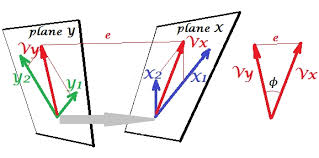
\includegraphics[height=3.5cm, width=6cm]{figures/canonical_correlation.jpg}
\end{center}
\end{figure}

$V_y$ and $V_x$ are selected to maximize:

\begin{itemize}
 \item Correlation (CCA)
 \item Squared Covariance (CIA)
       $$ \argmax_{p^i q^i} \text{cov}^2(Xp^i Yq^i)$$
\end{itemize}

\end{frame}

\begin{frame}\frametitle{Canonical Correlation}

\begin{itemize}
\item CCA has been used in omic data
\item The main limitation is that the number of features generally greatly exceeds the number of observations
\item Consequence 1: parameter estimation cannot be applied using standard methods
\item  Consequence 2: Most of markers are having no effect in the canonical axes (e.g. almost all components in a and b are 0)
\item Penalized (sparse) CCA has been proposed
\item Main advantages: More than two tables, easy interpretation (do not need computing p-values nor correcting for multiple comparisons)
\end{itemize}

\end{frame}



\begin{frame}\frametitle{Sparse canonical correlation}

\begin{figure}
\begin{center}
 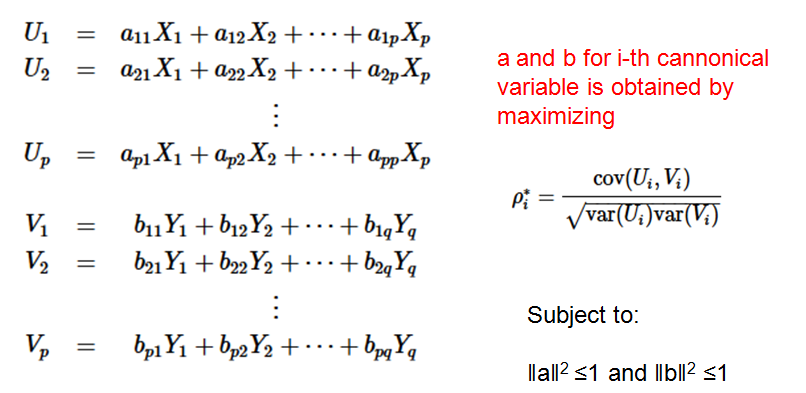
\includegraphics[height=5cm, width=8cm]{figures/mCCA.png}
\end{center}
\end{figure}

\end{frame}

\begin{frame}{Co-Inertia}

\begin{itemize}

  \item CIA does not requires an inversion step of the covariance matrix; thus, regularization or penalization implementation is not required
  \item CIA can deal with disperse variables
  \item CIA does consider quantitative or qualitative variables
  \item Can weight cases
  \item The method provides the RV coefficient. This is a measure of global similarity between the datasets, and is a number between 0 and 1. The closer it is to 1 the greater the global similarity between the two datasets. 
 \end{itemize}

\end{frame}



\begin{frame}[fragile]\frametitle{Canonical Correlation: gene expression and proteins}

\begin{knitrout}\footnotesize
\definecolor{shadecolor}{rgb}{0.969, 0.969, 0.969}\color{fgcolor}\begin{kframe}
\begin{alltt}
\hlkwd{require}\hlstd{(CCA)}
\hlstd{df1} \hlkwb{<-} \hlkwd{t}\hlstd{(breast_multi}\hlopt{$}\hlstd{RNAseq)[,}\hlnum{1}\hlopt{:}\hlnum{1000}\hlstd{]}
\hlstd{df2} \hlkwb{<-} \hlkwd{t}\hlstd{(breast_multi}\hlopt{$}\hlstd{RPPA)}
\end{alltt}
\end{kframe}
\end{knitrout}

\begin{knitrout}\footnotesize
\definecolor{shadecolor}{rgb}{0.969, 0.969, 0.969}\color{fgcolor}\begin{kframe}
\begin{alltt}
\hlstd{resCC} \hlkwb{<-} \hlkwd{cc}\hlstd{(df1, df2)}
\end{alltt}
\end{kframe}
\end{knitrout}


\begin{verbatim}
Error en chol.default(Bmat) : 
  la submatriz de orden 81 no es definida positiva
\end{verbatim}

\begin{knitrout}\footnotesize
\definecolor{shadecolor}{rgb}{0.969, 0.969, 0.969}\color{fgcolor}\begin{kframe}
\begin{alltt}
\hlstd{resRCC} \hlkwb{<-} \hlkwd{rcc}\hlstd{(df1, df2,} \hlnum{0.2}\hlstd{,} \hlnum{0.1}\hlstd{)}
\end{alltt}
\end{kframe}
\end{knitrout}

\begin{knitrout}\footnotesize
\definecolor{shadecolor}{rgb}{0.969, 0.969, 0.969}\color{fgcolor}\begin{kframe}
\begin{alltt}
\hlstd{regul} \hlkwb{<-} \hlkwd{estim.regul}\hlstd{(df1, df2)}
\hlstd{resRCC2} \hlkwb{<-} \hlkwd{rcc}\hlstd{(df1, df2, regul}\hlopt{$}\hlstd{lambda1, regul}\hlopt{$}\hlstd{lambda2)}
\end{alltt}
\end{kframe}
\end{knitrout}

\begin{knitrout}\footnotesize
\definecolor{shadecolor}{rgb}{0.969, 0.969, 0.969}\color{fgcolor}\begin{kframe}
\begin{alltt}
\hlkwd{plt.cc}\hlstd{(resRCC)}
\end{alltt}
\end{kframe}
\end{knitrout}

\end{frame}


\begin{frame}[fragile]\frametitle{Canonical Correlation: gene expression and proteins}

\begin{knitrout}\footnotesize
\definecolor{shadecolor}{rgb}{0.969, 0.969, 0.969}\color{fgcolor}

{\centering 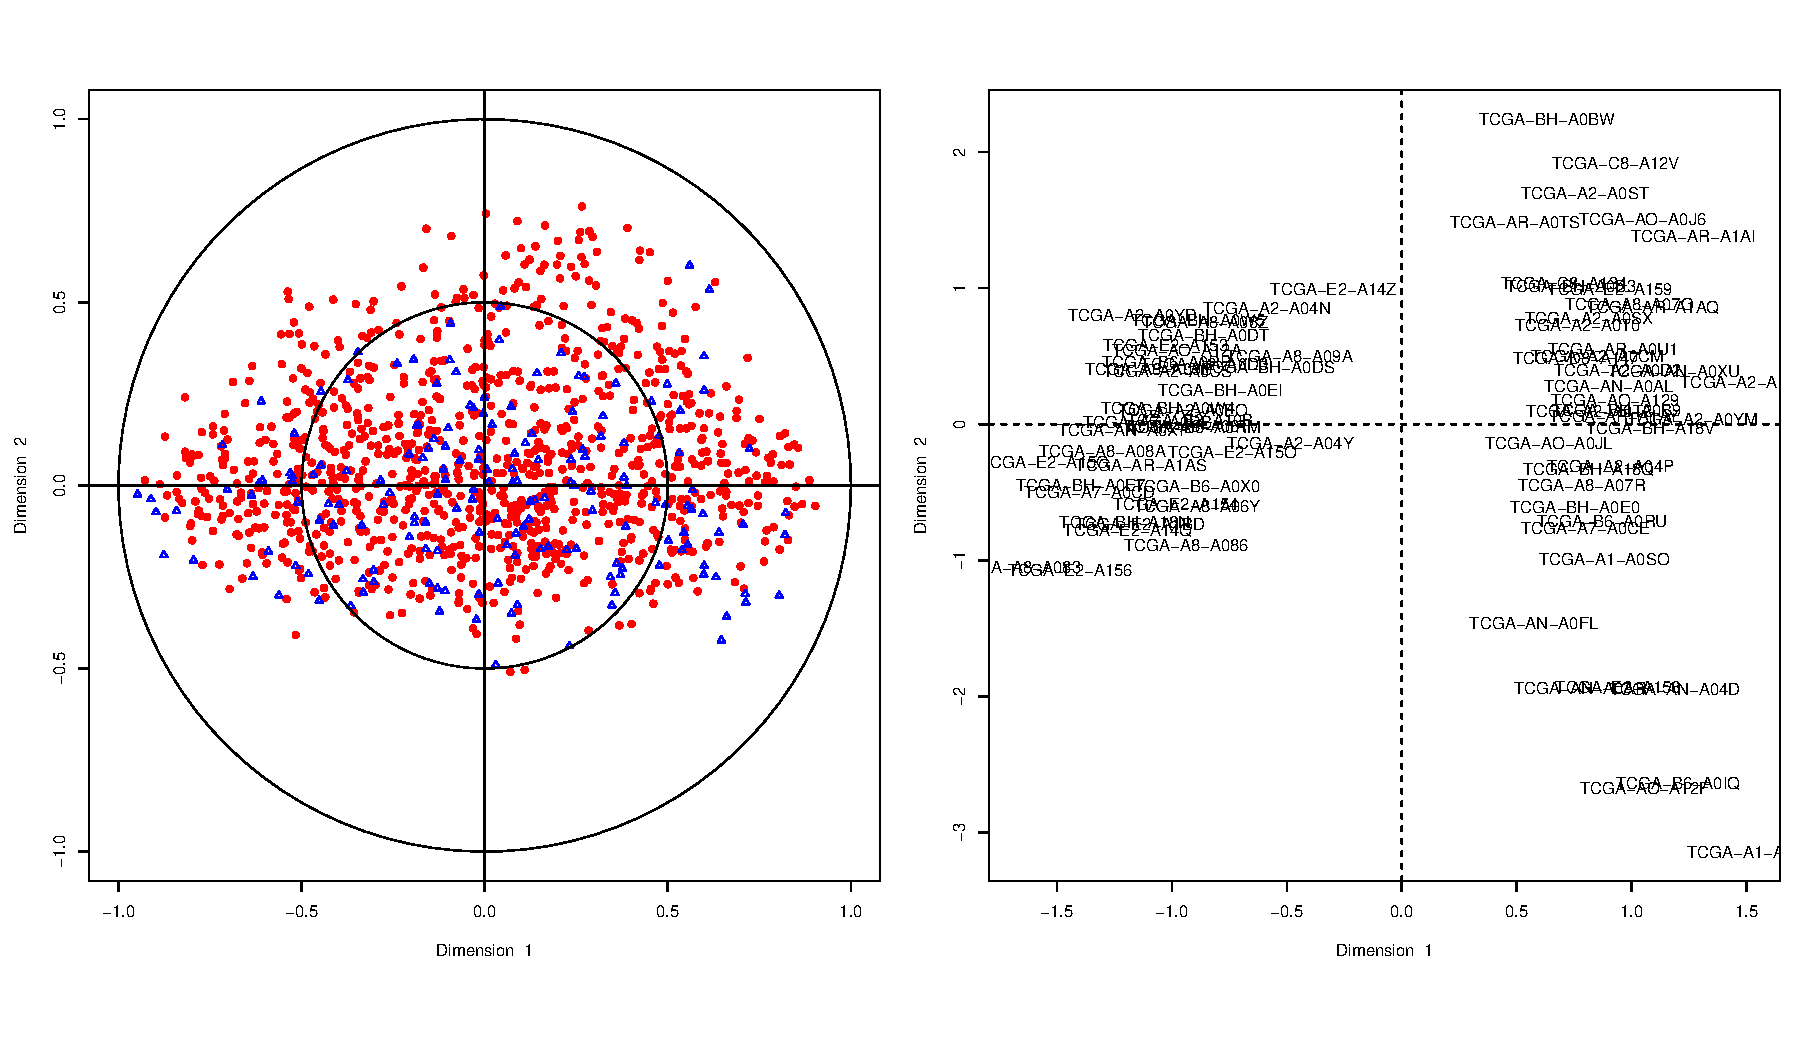
\includegraphics[width=2in]{figure/plot_rcc_out-1} 

}



\end{knitrout}

\end{frame}




\begin{frame}[fragile]\frametitle{Canonical Correlation: gene expression and proteins}

\begin{knitrout}\footnotesize
\definecolor{shadecolor}{rgb}{0.969, 0.969, 0.969}\color{fgcolor}\begin{kframe}
\begin{alltt}
\hlkwd{require}\hlstd{(PMA)}
\hlstd{ddlist} \hlkwb{<-} \hlkwd{list}\hlstd{(df1, df2)}
\hlstd{perm.out} \hlkwb{<-} \hlkwd{MultiCCA.permute}\hlstd{(ddlist,}
                             \hlkwc{type}\hlstd{=}\hlkwd{c}\hlstd{(}\hlstr{"standard"}\hlstd{,} \hlstr{"standard"}\hlstd{),}
                             \hlkwc{trace}\hlstd{=}\hlnum{FALSE}\hlstd{)}
\end{alltt}
\end{kframe}
\begin{kframe}\begin{alltt}
\hlstd{resMultiCCA} \hlkwb{<-} \hlkwd{MultiCCA}\hlstd{(ddlist,}
                        \hlkwc{penalty}\hlstd{=perm.out}\hlopt{$}\hlstd{bestpenalties,}
                        \hlkwc{ws}\hlstd{=perm.out}\hlopt{$}\hlstd{ws.init,}
                        \hlkwc{type}\hlstd{=}\hlkwd{c}\hlstd{(}\hlstr{"standard"}\hlstd{,} \hlstr{"standard"}\hlstd{),}
                        \hlkwc{ncomponents}\hlstd{=}\hlnum{1}\hlstd{,} \hlkwc{trace}\hlstd{=}\hlnum{FALSE}\hlstd{,} \hlkwc{standardize}\hlstd{=}\hlnum{TRUE}\hlstd{)}
\end{alltt}
\end{kframe}
\end{knitrout}

NOTE: setting {\tt type} equal to "ordered" allows to consider that features are correlated (e.g. genomic regions) 
\end{frame}


\begin{frame}[fragile]\frametitle{Canonical Correlation: gene expression and proteins}

\begin{knitrout}\scriptsize
\definecolor{shadecolor}{rgb}{0.969, 0.969, 0.969}\color{fgcolor}\begin{kframe}
\begin{alltt}
\hlkwd{rownames}\hlstd{(resMultiCCA}\hlopt{$}\hlstd{ws[[}\hlnum{1}\hlstd{]])} \hlkwb{<-} \hlkwd{colnames}\hlstd{(df1)}
\hlkwd{rownames}\hlstd{(resMultiCCA}\hlopt{$}\hlstd{ws[[}\hlnum{2}\hlstd{]])} \hlkwb{<-} \hlkwd{colnames}\hlstd{(df2)}
\hlkwd{head}\hlstd{(resMultiCCA}\hlopt{$}\hlstd{ws[[}\hlnum{1}\hlstd{]])}
\end{alltt}
\begin{verbatim}
##                 [,1]
## CREB3L1   0.03812575
## PNMA1     0.04078831
## MMP2      0.02402715
## C10orf90 -0.02896362
## GPR98     0.04723420
## APBB2     0.06279879
\end{verbatim}
\begin{alltt}
\hlkwd{head}\hlstd{(resMultiCCA}\hlopt{$}\hlstd{ws[[}\hlnum{2}\hlstd{]])}
\end{alltt}
\begin{verbatim}
##                    [,1]
## c.Myc       -0.07099252
## HER3         0.02652238
## XBP1         0.00000000
## Fibronectin  0.01527691
## PAI.1       -0.02319958
## p21          0.02415011
\end{verbatim}
\end{kframe}
\end{knitrout}
\end{frame}





\begin{frame}[fragile]\frametitle{Co-inertia: gene expression and proteins}

Let us load required packages (coinertia and multiple coinertia)
\begin{knitrout}\footnotesize
\definecolor{shadecolor}{rgb}{0.969, 0.969, 0.969}\color{fgcolor}\begin{kframe}
\begin{alltt}
\hlkwd{library}\hlstd{(made4)}
\hlkwd{library}\hlstd{(omicade4)}
\end{alltt}
\end{kframe}
\end{knitrout}

\begin{knitrout}\footnotesize
\definecolor{shadecolor}{rgb}{0.969, 0.969, 0.969}\color{fgcolor}\begin{kframe}
\begin{alltt}
\hlstd{resCIA} \hlkwb{<-} \hlkwd{cia}\hlstd{(breast_multi}\hlopt{$}\hlstd{RNAseq, breast_multi}\hlopt{$}\hlstd{RPPA)}
\end{alltt}
\end{kframe}
\end{knitrout}

\begin{knitrout}\footnotesize
\definecolor{shadecolor}{rgb}{0.969, 0.969, 0.969}\color{fgcolor}\begin{kframe}
\begin{alltt}
\hlkwd{plot}\hlstd{(resCIA,} \hlkwc{classvec}\hlstd{=group,} \hlkwc{nlab}\hlstd{=}\hlnum{3}\hlstd{,} \hlkwc{clab}\hlstd{=}\hlnum{0}\hlstd{,} \hlkwc{cpoint}\hlstd{=}\hlnum{3} \hlstd{)}
\end{alltt}
\end{kframe}
\end{knitrout}

\end{frame}



\begin{frame}[fragile]\frametitle{Co-inertia: gene expression and proteins}

\begin{figure}
\begin{center}
 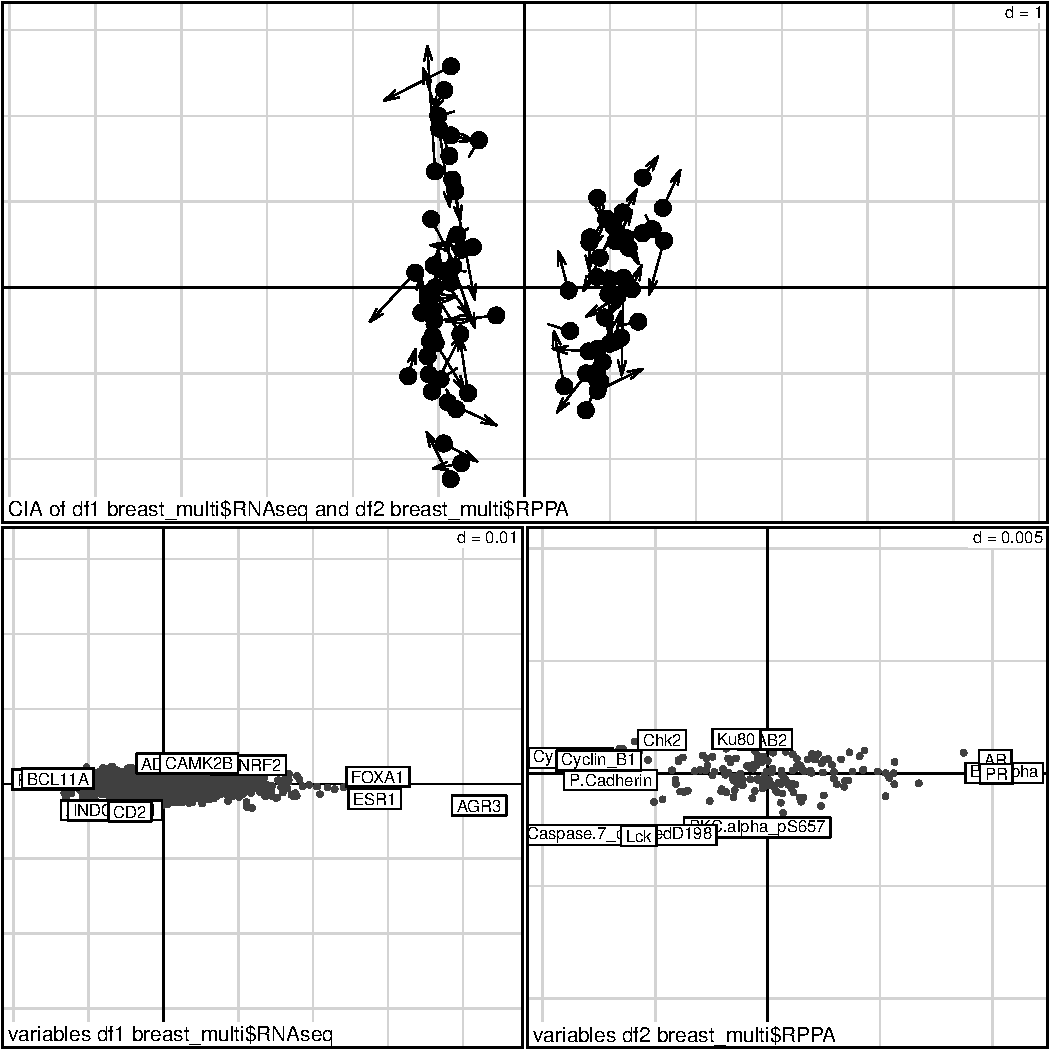
\includegraphics[width=6cm]{figure/plot_cia-1}
\end{center}
\end{figure}

\end{frame}


\begin{frame}[fragile]\frametitle{Co-inertia: gene expression and proteins}

Top-5 features of the first axis (positive side) can be retrieve by

\footnotesize 
\begin{knitrout}\footnotesize
\definecolor{shadecolor}{rgb}{0.969, 0.969, 0.969}\color{fgcolor}\begin{kframe}
\begin{alltt}
\hlkwd{topVar}\hlstd{(resCIA,} \hlkwc{axis}\hlstd{=}\hlnum{1}\hlstd{,} \hlkwc{topN}\hlstd{=}\hlnum{5}\hlstd{,} \hlkwc{end}\hlstd{=}\hlstr{"positive"}\hlstd{)}
\end{alltt}
\begin{verbatim}
##   ax1_df1_positive ax1_df2_positive
## 1             AGR3         ER.alpha
## 2            FOXA1               PR
## 3             ESR1               AR
## 4             AGR2           INPP4B
## 5          C1orf64            GATA3
\end{verbatim}
\end{kframe}
\end{knitrout}

\end{frame}



\begin{frame}[fragile]\frametitle{Co-inertia: gene expression and proteins}

Top-5 features of the first axis (negative side) can be retrieve by

\footnotesize 
\begin{knitrout}\footnotesize
\definecolor{shadecolor}{rgb}{0.969, 0.969, 0.969}\color{fgcolor}\begin{kframe}
\begin{alltt}
\hlkwd{topVar}\hlstd{(resCIA,} \hlkwc{axis}\hlstd{=}\hlnum{1}\hlstd{,} \hlkwc{topN}\hlstd{=}\hlnum{5}\hlstd{,} \hlkwc{end}\hlstd{=}\hlstr{"negative"}\hlstd{)}
\end{alltt}
\begin{verbatim}
##   ax1_df1_negative      ax1_df2_negative
## 1            ROPN1             Cyclin_E1
## 2           ROPN1B             Cyclin_B1
## 3           BCL11A            P.Cadherin
## 4             ART3                  MSH6
## 5            SFRP1 Caspase.7_cleavedD198
\end{verbatim}
\end{kframe}
\end{knitrout}

\end{frame}



\begin{frame}[fragile]\frametitle{More than two tables}


\begin{knitrout}\footnotesize
\definecolor{shadecolor}{rgb}{0.969, 0.969, 0.969}\color{fgcolor}\begin{kframe}
\begin{alltt}
\hlstd{resMCIA} \hlkwb{<-} \hlkwd{mcia}\hlstd{( breast_multi[} \hlkwd{c}\hlstd{(}\hlnum{1}\hlstd{,}\hlnum{3}\hlstd{,}\hlnum{4}\hlstd{,}\hlnum{5}\hlstd{,}\hlnum{6}\hlstd{,}\hlnum{7}\hlstd{) ] )}
\end{alltt}
\end{kframe}
\end{knitrout}


\begin{knitrout}\footnotesize
\definecolor{shadecolor}{rgb}{0.969, 0.969, 0.969}\color{fgcolor}\begin{kframe}
\begin{alltt}
\hlkwd{plot}\hlstd{(resMCIA,} \hlkwc{axes}\hlstd{=}\hlnum{1}\hlopt{:}\hlnum{2}\hlstd{,} \hlkwc{sample.lab}\hlstd{=}\hlnum{FALSE}\hlstd{,} \hlkwc{sample.legend}\hlstd{=}\hlnum{FALSE}\hlstd{,}
     \hlkwc{phenovec}\hlstd{=group,} \hlkwc{gene.nlab}\hlstd{=}\hlnum{2}\hlstd{,}
     \hlkwc{df.color}\hlstd{=}\hlkwd{c}\hlstd{(}\hlstr{"cyan"}\hlstd{,} \hlstr{"magenta"}\hlstd{,} \hlstr{"red4"}\hlstd{,} \hlstr{"brown"}\hlstd{,}\hlstr{"yellow"}\hlstd{,} \hlstr{"orange"}\hlstd{),}
     \hlkwc{df.pch}\hlstd{=}\hlnum{2}\hlopt{:}\hlnum{7}\hlstd{)}
\end{alltt}
\end{kframe}
\end{knitrout}
\end{frame}


\begin{frame}[fragile]\frametitle{More than two tables}

\begin{figure}
\begin{center}
 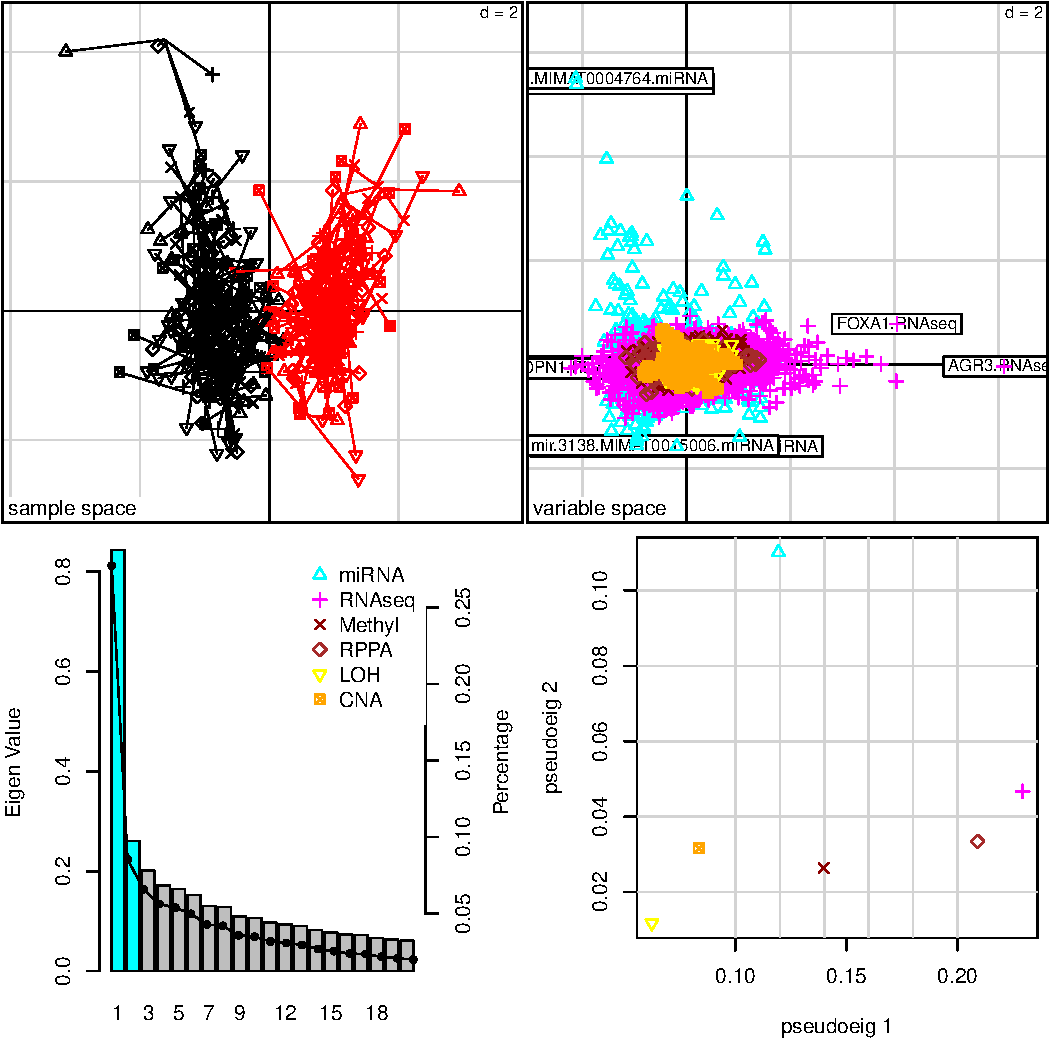
\includegraphics[width=5.5cm]{figure/plot_mcia-1}
\end{center}
\end{figure}

\end{frame}

\begin{frame}[fragile]\frametitle{More than two tables}

Top-5 features of the first axis (positive side) can be retrieve by

\scriptsize 
\begin{knitrout}\footnotesize
\definecolor{shadecolor}{rgb}{0.969, 0.969, 0.969}\color{fgcolor}\begin{kframe}
\begin{alltt}
\hlkwd{topVar}\hlstd{(resMCIA,} \hlkwc{end}\hlstd{=}\hlstr{"positive"}\hlstd{,} \hlkwc{axis}\hlstd{=}\hlnum{1}\hlstd{,} \hlkwc{topN}\hlstd{=}\hlnum{5}\hlstd{)}
\end{alltt}
\begin{verbatim}
##                ax1_miRNA_positive ax1_RNAseq_positive ax1_Methyl_positive
## 1 hsa.mir.4254.MIMAT0016884.miRNA         AGR3.RNAseq   cg08097882.Methyl
## 2 hsa.mir.3945.MIMAT0018361.miRNA        FOXA1.RNAseq   cg09952204.Methyl
## 3 hsa.mir.302b.MIMAT0000715.miRNA         ESR1.RNAseq   cg04988423.Methyl
## 4 hsa.mir.1265.MIMAT0005918.miRNA         AGR2.RNAseq   cg00679738.Methyl
## 5 hsa.mir.3171.MIMAT0015046.miRNA      C1orf64.RNAseq   cg12601757.Methyl
##   ax1_RPPA_positive ax1_LOH_positive ax1_CNA_positive
## 1     ER.alpha.RPPA        X4006.LOH        X8374.CNA
## 2           AR.RPPA        X4007.LOH        X8381.CNA
## 3           PR.RPPA        X4008.LOH        X8382.CNA
## 4       INPP4B.RPPA        X4009.LOH        X8383.CNA
## 5        GATA3.RPPA        X4010.LOH        X8384.CNA
\end{verbatim}
\end{kframe}
\end{knitrout}

\end{frame}



\begin{frame}[fragile]\frametitle{More than two tables}

\begin{knitrout}\footnotesize
\definecolor{shadecolor}{rgb}{0.969, 0.969, 0.969}\color{fgcolor}\begin{kframe}
\begin{alltt}
\hlkwd{plot}\hlstd{(resMCIA}\hlopt{$}\hlstd{mcoa}\hlopt{$}\hlstd{cov2,}  \hlkwc{xlab} \hlstd{=} \hlstr{"pseudoeig 1"}\hlstd{,}
     \hlkwc{ylab} \hlstd{=} \hlstr{"pseudoeig 2"}\hlstd{,} \hlkwc{pch}\hlstd{=}\hlnum{19}\hlstd{,} \hlkwc{col}\hlstd{=}\hlstr{"red"}\hlstd{)}
\hlkwd{text}\hlstd{(resMCIA}\hlopt{$}\hlstd{mcoa}\hlopt{$}\hlstd{cov2,} \hlkwc{labels}\hlstd{=}\hlkwd{rownames}\hlstd{(resMCIA}\hlopt{$}\hlstd{mcoa}\hlopt{$}\hlstd{cov2),}
     \hlkwc{cex}\hlstd{=}\hlnum{1.4}\hlstd{,} \hlkwc{adj}\hlstd{=}\hlnum{0}\hlstd{)}
\end{alltt}
\end{kframe}
\end{knitrout}

\begin{figure}
\begin{center}
 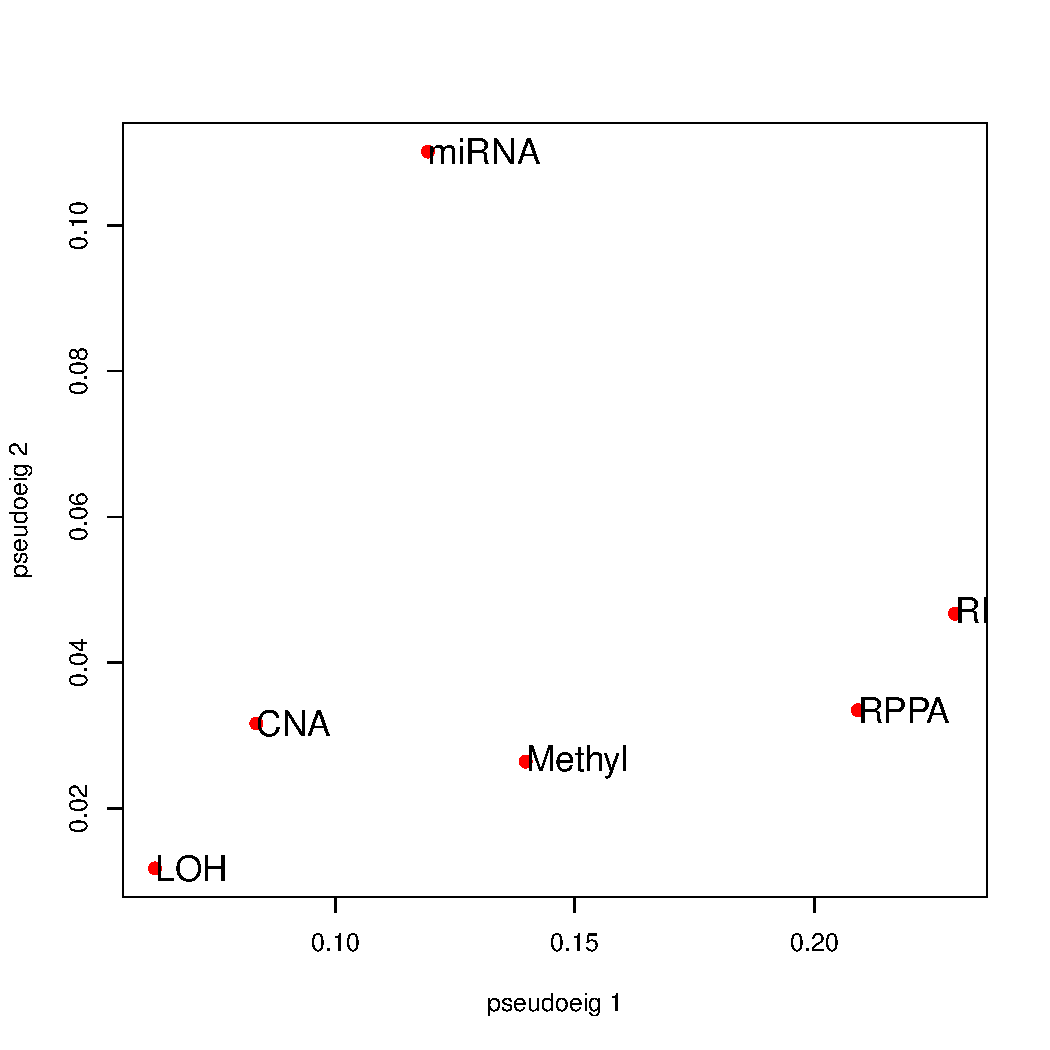
\includegraphics[width=5.5cm]{figure/plot_eigen-1}
\end{center}
\end{figure}

\end{frame}


\begin{frame}\frametitle{Take home messages}

\begin{description}[labelwidth=\widthof{\textbf{Canonical correlation}}]
 \item[Correlation] Y = X
 \item[Multiple correlation] $Y = X_1 X_2 X_3 \cdots X_k$
 \item[Canonical correlation] $Y_1 Y_2 Y_3 \cdots Y_j = X_1 X_2 X_3 \cdots X_k$
\end{description}

\begin{itemize}
  \item Co-inertia analysis (CIA) is similar to CCA but it optimizes the squared covariance between the eigenvectors while CC optimizes
        the correlation. 
  \item CIA can be applied to datasets where the number of variables (genes) far exceeds the number of samples (arrays) such is the case in several omic data, while CCA requires a regularized version to be implemented. 
  \item Sparse and reguralized methods requires a tuning parameter. This makes these methods computing demanding.
\end{itemize}


\end{frame}



\begin{frame}\frametitle{Take home messages}
\begin{itemize}
  \item Multivariate methods are purely descriptive methods that do not test a hypothesis to generate a p-value.
  \item They are not optimized for variable of biomarkers discovery, though the introduction of sparsity in variable loadings may help in the selection of variables forn downstream analyses.
  \item Number of variables in omic data is a challenge to tradicional visualization tools. New {\tt R} packages including {\tt ggord} are being developed to address this issue.
  \item Dynamic visualization is possible using {\tt ggvis}, {\tt ploty}, {\tt explor} and other packages.
  \item Projection in the same space of variable annotation (GO or Reactome) may help to determine gene sets or patwhays associated with our traits.

\end{itemize}
\end{frame}


\section{Recommended lectures}

\begin{frame}\frametitle{Recommended lectures}

\footnotesize

\begin{itemize}
\item Richmond et al. (2016). Challenges and novel approaches for investigating molecular mediation. Hum Mol Genet, 25(R2):R149-R156.
\item Millstein et al. (2009). Disentangling molecular relationships with a causal inference test. BMC Bioinf, 10:23.
\item Ebrahim and Smith (2008). Mendelian randomization: can genetic epidemiology help redress the failure of observational epidemiology?. Hum Genet, 123:15-33.
\item Liu et al. (2013). Epifenome-wide association data implicate DNA methylation as an intermediary of genetic risk in rheumatoid arthritis. Nat Biotech, 31(2):142-148.
\item Voight et al. (2012). Plasma HDL cholesterol and risk of myocardial infarction: a mendelian randomisation study. Lancet, 380(9841): 572-580.
\item Meng et al. (2014). A multivariate approach to the integration of multi-omics datasets. BMC Bioinf, 15:162.
\item Witten et al. (2009). A Penalized Matrix Decomposition, with Applications to Sparse Principal Components and Canonical Correlation Analysis. Biostatistics, 10(3):515-34.
\item Meng et al (2016). Dimension reduction techniques for the integrative analysis of multi-omics data. Brief Bioinform, 17(4): 628-641. 
\end{itemize}
\end{frame}



\end{document}















